\documentclass[letterpaper, 10pt, conference]{ieeeconf}  % 
\IEEEoverridecommandlockouts                              % This command is only needed if 
                                                          % you want to use the \thanks command
\overrideIEEEmargins    
\usepackage{cite}

\usepackage{algorithmic}

\usepackage{textcomp}

\usepackage{comment}

%\usepackage{graphicx}      % include this line if your document contains figures
%\usepackage{natbib}        % required for bibliography
%===============================================================================
% Needed to meet printer requirements.
 \usepackage{latexsym,amssymb,amsfonts}
\usepackage[applemac]{inputenc}
\usepackage{rotating}
\usepackage{cite}
%\usepackage{graphicx}
\usepackage{epstopdf}
% \usepackage{subfigure}
%\usepackage{color}
%\usepackage{xcolor}
%
%\usepackage{color}
\usepackage[dvipsnames]{xcolor}
%
\usepackage[normalem]{ulem}
\usepackage{isolatin1}
%\usepackage{caption}
\usepackage{subcaption} 
\usepackage{booktabs}

%\usepackage{array,multirow,makecell}
%\usepackage{placeins}
%\usepackage{stackengine}
%\usepackage{hyperref}
\usepackage{fancybox}
\usepackage{colortbl}
\usepackage{float}
\usepackage{comment}
\usepackage{mathdots}
%\usepackage{lmodern}
%%%%%%%%%%%%%%%%%%%%%%%%%%%%%%%%%%%%%%%%%%%%%%%%%%%%%%%%%
\usepackage{dblfloatfix}
\usepackage{kantlipsum}
\usepackage{dblfloatfix}    % To enable figures at the bottom of page
\usepackage{graphicx} % [demo] option for empty figure
\usepackage{placeins}
\usepackage{marginnote}
\usepackage{url}
\usepackage{hyperref}
\usepackage{fancybox}
%\usepackage{empheq}
\usepackage[overload]{empheq}

\usepackage{bm}

%%%%%%%%%%%%%%%%%%%%%%%%%%%%%%%%%%%%%%%%%%%%%%%%%%%%%%%%%
\usepackage{tikz}
\usetikzlibrary{circuits.ee.IEC}
\usepackage[european resistor, european voltage, european current]{circuitikz}
\usetikzlibrary{arrows, shapes, positioning}
\usetikzlibrary{decorations.markings, decorations.pathmorphing,
decorations.pathreplacing}
\usetikzlibrary{calc,patterns,shapes.geometric}
\usetikzlibrary{shapes.multipart, positioning, patterns, backgrounds}
\tikzstyle{titlebox}=[rectangle,inner sep=10pt,inner ysep=10pt,draw]%
\usetikzlibrary{arrows.meta}
\usetikzlibrary{matrix, fit}

%%%%%%%%%%%%%%%%%%%%%%%%%%%%%%%%%%%%%%%%%%%%%%%%%%%%%%%%%%%%%

\def\blacksquare{\hbox{\vrule width 4pt height 4pt depth 0pt}}
\def\square{\hbox{\vrule\barox{\hrule\phantom{o}\hrule}\vrule}}
\def\qed{\hfill \square}
\def\qedp{\rightline{$\blacksquare$}}
\def\EXPT{\mathop{{\rm E}}}
\def\MIN{\mathop{{\rm min}}}
\def\MAX{\mathop{{\rm max}}}
\def\LIM{\mathop{{\longrightarrow}}}
\def\UNION{\mathop{\bigcup}}
\def\INTERSECT{\mathop{\bigcap}}
\def\ARGMIN{\mathop{{\rm argmin}}}
\def\ARGMAX{\mathop{{\rm argmax}}}
\def\TOUND{\mathop{\longrightarrow}}
\def\col#1{\mathop{{\rm col}\,\left(\,#1\,\right)}}
\def\eqref#1{(\ref{#1})}
\def\rank{\mathop{{\rm rank}}}

\newcommand{\widebox}[2][0.5em]{\fbox{\hspace{#1}$\displaystyle #2$\hspace{#1}}}



\def\rank{\mathop{{\rm rank}}}

% User definition from Shengya
\def\V{\mathcal{V}} % the set of vehicle
\def\E{\mathcal{E}} % the set of edge
\def\G{\mathcal{G}} % graph
\def\A{\mathcal{A}} % adjacency matrix 
\def\W{\mathcal{W}} % weighted adjacency matrix
\def\L{\mathcal{L}} % Laplacian matrix
\def\N{\mathcal{N}} % neighbors
\def\LO{\mathcal{LO}} % the set of observer
\def\DO{\mathcal{DO}} % the set of observer
\def\diag#1{\mathop{{\rm diag}\,\left(\,#1\,\right)}}
\def\ST{\mathcal{ST}} % Self trust
\def\LT{\mathcal{LT}} % Local trust
\def\DT{\mathcal{DT}} % Distributed trust 
\def\VT{\mathcal{VT}} % Vehicle trust 
\def\AT{\mathcal{AT}} % Aggregation trust
\def\T{\mathcal{T}} % Aggregation trust
\def\O{\mathcal{O}} % opinion


% User Defined Color based on RGB
\definecolor{userblue}{RGB}{31,119,180}
\definecolor{userorange}{RGB}{255,127,14}
\definecolor{usergreen}{RGB}{44,160,44}
\definecolor{userpurple}{RGB}{148,103,189}

\definecolor{blue1}{RGB}{31,119,180}    % 车辆/物理层
\definecolor{orange1}{RGB}{255,127,14}  % 本地观测器
\definecolor{green1}{RGB}{44,160,44}    % 信息层/通信
\definecolor{purple1}{RGB}{148,103,189} % 分布式观测器
\definecolor{rose1}{RGB}{227, 119, 194}

%%%
\newtheorem{prb}{\it Problem}%[section]
\newtheorem{theorem}{\it Theorem}%[section]
\newtheorem{lemma}{\it Lemma}%[section]
\newtheorem{definition}{\it Definition}
\newtheorem{remark}{\it Remark}%[section]
\newtheorem{assumption}{\it Assumption}%[section]
\newtheorem{example}{\it Example}%[section]b
\newtheorem{annex}{\it Annex}%[section]b
\newtheorem{prop}{\it Proposition}%[section]b

\newtheorem{alert}{\color{red}\it Alert Remark}
% \newtheorem{proof}{\it Proof}%[section]b




\def\BibTeX{{\rm B\kern-.05em{\sc i\kern-.025em b}\kern-.08em
    T\kern-.1667em\lower.7ex\hbox{E}\kern-.125emX}}

\tikzset{global scale/.style={
    scale=#1,
    every node/.append style={scale=#1}
  }
}

\begin{document}


\title{\bf Resilience in Distributed
 Observer based on Trust for Connected Vehicle }
\author{Q.H. Nguyen$^{1,2}$, Shengya Meng $^{1}$, H. Rafaralahy $^{1}$, M. Haddad $^{2}$, A. Zemouche $^{1}$
%
\thanks{This work was supported by SEGULA Engineering. H. Rafaralahy and A. Zemouche would like to acknowledge the ANR agency for its partial financial support under the project ArtISMo ANR-20-CE48-0015.
}
%
\thanks{$^{1}$ Universit\'e de Lorraine, CNRS, CRAN, F-57000 Metz, France~(e-mail: \protect\url{ali.zemouche@univ-lorraine.fr}).}
%
\thanks{$^{2}$ SEGULA Engineering, 19 rue d'Arras, 92000 Nanterre, France~(e-mail: \protect\url{madjid.haddad@segula.fr}).}
%
\thanks{All relevant CARLA resources have been made available in \protect\href{https://github.com/kslhuy/CACC_UIO_simulink}{GitHub}.}
}
\maketitle

\begin{abstract}
The distributed driving state estimation problem is critical for optimizing vehicle platoon performance. This paper proposes a novel trust layer that evaluates data from platoon members by analyzing discrepancies between their reported and actual behaviors. Leveraging this layer, a trustworthiness-based neighbor set is constructed, informing the design of a weight gain matrix for a distributed observer. This method enables resilient estimation, maintaining stability despite unreliable data. The paper also derives sufficient conditions for the stability of the estimation error dynamics. By enhancing the robustness and reliability of state estimation, this approach advances the safety and efficiency of autonomous vehicle platoons. Testing across multiple attack cases, such as bogus messages, replay attacks, and denial-of-service (DoS) attacks, confirms the method's strong performance, consistently ensuring accurate estimation and platoon stability.
\end{abstract}

\begin{keywords}
Distributed observers, secure estimation, lyapunov stability, cyber-attack.
\end{keywords}


\begin{figure}
\centering
    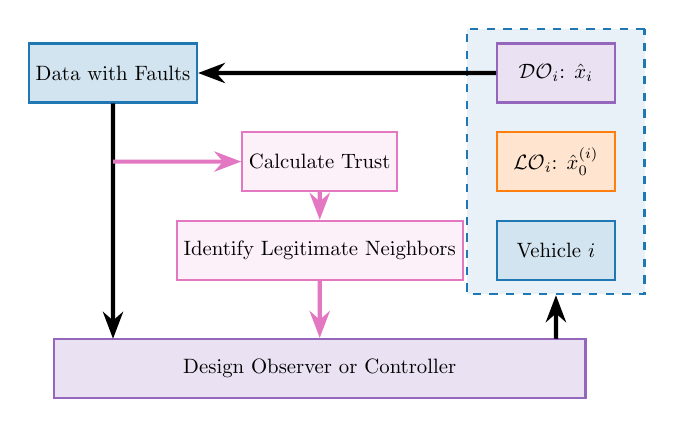
\begin{tikzpicture}[global scale = 0.75,
    vehicle/.style={draw=blue1, fill=blue1!20, thick, minimum width=2cm, minimum height=1cm},
    localobs/.style={draw=orange1, fill=orange1!20, thick, minimum width=2cm, minimum height=1cm},
    distobs/.style={draw=purple1, fill=purple1!20, thick, minimum width=2cm, minimum height=1cm},
    sigarrow/.style={-Stealth, line width=1.5pt, color=black},
    commarrow/.style={
    double,
    double distance=1pt,
    line width=0.7pt,
    draw=green1,
    -Stealth
    },
    physics/.style={draw=blue1, shape=rectangle, fill=blue1!10,line width=0.75pt,dashed,minimum width=3cm, minimum height=4.5cm}, %
    trustlayer/.style={draw=rose1, shape=rectangle, fill=rose1!10,thick,minimum width=13cm, minimum height=1cm},
    trust/.style={draw=rose1, shape=ellipse, fill=rose1!10,thick,minimum width=1.5cm, minimum height=1cm}
]

  %   		\draw [help lines,step=0.5cm] (0,0) grid (18,10); % 辅助网格 
		% % 画x和y轴坐标
		% \draw[stealth-,line width=2pt] (0,0)--(15,0);
		% % 画刻度
		% \foreach \x in {0,1,...,5}
		% {
		% 	\draw[xshift=\x cm] (0,0) -- (0,0.5);
		% };  
		% % 标坐标原点
		% \node[below] at (0,0){0};
		% %标x轴刻度值
		% \foreach \y in {1,2,...,18}
		% \node[below] at(\y,0){\y};

        \node[physics,line width=0.75pt,minimum width=3cm, minimum height=4.5cm, name = phy] at(14,1.5) { };
        \node[vehicle,name=host] at(14,0) {Vehicle $i$};
        \node[localobs,name=LOh] at(14,1.5) {$\LO_{i}$: $\hat{x}_{0}^{(i)}$};
        \node[distobs,name=DOh] at(14,3) {$\DO_{i}$: $\hat{x}_{i}$};

        \node[vehicle, name=data] at(6.5,3) {Data with Faults};
        \node[distobs, name=design,minimum width=9cm] at(10,-2) {Design Observer or Controller};

        \node[trust,shape=rectangle, name=trust] at(10,1.5) {Calculate Trust}; 
        \node[trust,shape=rectangle, name=id] at(10,0) {Identify Legitimate Neighbors};

        \draw[sigarrow] (DOh) -- (data);
        
        \draw[sigarrow] (data) --(6.5,-1.5);
        \draw[sigarrow] (14,-1.5) -- (phy);

        \draw[sigarrow, rose1,](6.5,1.5) -- (trust);
        \draw[sigarrow, rose1,](trust) -- (id);
        \draw[sigarrow, rose1,](id) -- (design);
    \end{tikzpicture}
\end{figure}


\section{Introduction}\label{sec_introduction}

In recent years, the development of autonomous and connected vehicles has gained significant attention due to their potential to enhance road safety, reduce traffic congestion, and improve fuel efficiency. A critical aspect of these systems is the ability to coordinate multiple vehicles effectively, often organized in platoons, where vehicles follow a leader while maintaining a desired distance from each other. To achieve optimal performance in such platoons, accurate estimation of the global driving state is essential. This involves reconstructing the states of all vehicles in the platoon based on local measurements and communicated data. However, the distributed nature of these systems introduces vulnerabilities, particularly in the presence of malicious or faulty agents that can disrupt coordination and compromise the integrity of the state estimation process.
The distributed driving state estimation problem is pivotal for ensuring the stability and efficiency of vehicle platoons. Traditional approaches often assume that all agents are cooperative and trustworthy, which is not always realistic in real-world scenarios. Malicious agents can manipulate the data they share, leading to incorrect state estimates and potentially catastrophic consequences for the platoon. Therefore, developing resilient estimation techniques that can handle such adversarial conditions is of paramount importance.

In this paper, we address the challenge of resilient distributed state estimation in vehicle platoons. Our approach introduces a novel trust model that evaluates the reliability of data from platoon members by assessing the divergence between their reported behavior and their actual behavior. This trust model enables the construction of a dynamic set of neighbors based on trustworthiness, which is then used to design a weight gain matrix for a distributed observer. By incorporating this trust-based mechanism, we achieve resilient estimation that can withstand the presence of malicious agents. Furthermore, we provide necessary and sufficient conditions to ensure the stability of the estimation error dynamics, offering a robust theoretical foundation for our approach.

Our contributions in this paper are threefold:
\begin{enumerate}
    \item \textbf{Problem Formulation:} Formal definition of the resilient distributed state estimation problem for vehicle platoons under adversarial conditions
    
    \item \textbf{Trust Model:} Novel behavioral divergence metric for quantifying agent trustworthiness and enabling dynamic neighbor selection
    
    \item \textbf{Observer Design:} Trust-aware distributed observer with provable stability guarantees and empirical validation
\end{enumerate}

This paper unfolds as follows: Section \ref{sec_related_work} reviews related work. Section \ref{sec_related_work} formulates the problem. Section \ref{sec_vehiclemodel} presents the system model and problem formulation. Section \ref{sec_Distributed Observer} details the distributed observer, Section \ref{sec_Evolution_trust} presents the trust framework, Section \ref{sec_Weigth_Design} designs the observer weights and provides the stability analysis. Section \ref{sec_simulation} discusses simulations in different scenarios, also the application of the estimated state to the controller. Section \ref{sec_conclusion} concludes with future directions.

\section{Related Work}\label{sec_related_work}
\textcolor{blue}{Everything here needs to change carefully and corrected}

\textcolor{red}{The security of cyber-physical systems (CPS) and distributed multi-agent systems (DMAS), such as vehicle platooning with vehicle-to-vehicle (V2V) communication, is a critical research area due to the safety implications of these systems. A significant challenge lies in detecting and mitigating cyber-attacks that compromise state estimation and control. This section explores key techniques for attack detection and mitigation, with a focus on their application to CPS and DMAS.
}

\subsection*{Detection}
% Summarizing detection approaches
Most literature focuses on detecting the presence of attacks in CPS and DMAS, with advanced methods also identifying the source, type, and severity of the attack. These capabilities are essential for enabling effective mitigation and maintaining system integrity.

\begin{itemize}
    \item \textbf{Observer-Based Detection}: 
    % Describing observer-based methods
    Observer-based techniques compare the estimated states from a system model (e.g., an observer) with actual measurements to detect anomalies \cite{2_obs_Angelo , SHAMES20112757}. In vehicle platooning, an observer can predict the expected behavior of neighboring vehicles based on their dynamics and flag deviations as potential attacks \cite{KF_chisquare_meusure}. However, a key drawback is that these methods may use faulty data from compromised neighbors, leading to inaccurate estimations and potential false positives or missed detections.

    \item \textbf{Consensus-Based Detection}: 
    % Explaining consensus-based approaches
    These methods leverage multiple sensors or agents to cross-validate measurements \cite{Guitao_multi_mesure}. By comparing data across different sources, a common value or behavior is established, and significant deviations suggest an attack. For instance, in a platoon, if most vehicles report consistent spacing but one diverges, it may indicate malicious behavior. The limitation is the assumption that a majority of agents remain uncompromised, which may not hold in large-scale attacks.

    \item \textbf{Trust-Based Detection}: 
    % Detailing trust-based techniques
    Trust-based approaches assess the reliability of agents or data sources, often assigning trust scores to neighbors.
    \begin{enumerate}
        \item \textit{Physical Connectivity-Based Methods}: These analyze physical signals, such as device fingerprints or signal characteristics, to verify authenticity and assign trust scores. For example, unique wireless communication fingerprints can distinguish legitimate vehicles from spoofed ones \cite{trust_physic_connecte}.
        \item \textit{Statistical Methods}: These compare communicated data with locally observed data (e.g., from onboard sensors) to detect inconsistencies indicative of attacks. 
    \end{enumerate}
    % Highlighting relevance to consensus and observers
    Misbehavior detection based on trust is particularly useful in consensus problems and can enhance observer-based methods by filtering unreliable inputs. However, these techniques may require significant computational resources or historical data, posing challenges in dynamic settings like platooning.
\end{itemize}

% Noting advanced detection capabilities
Advanced detection techniques provide additional insights (e.g., attack source or type), which are critical for tailoring mitigation strategies. Trust scores for neighbors, derived from these methods, further refine detection accuracy.

\subsection*{Mitigation}
% Connecting mitigation to detection
Mitigation strategies depend heavily on the detection step, with more advanced algorithms providing richer information to guide responses. Common approaches include:

\begin{enumerate}
    \item \textbf{Switching to a Worst-Case Mode}: 
    % Describing safe mode switching
    A standard response is to revert to a safe operational mode, such as switching from cooperative adaptive cruise control (CACC) to adaptive cruise control (ACC). ACC relies solely on local sensors, avoiding compromised V2V data. While effective, this sacrifices cooperative benefits and may degrade performance unnecessarily if only a subset of data is faulty.

    \item \textbf{Incorporating Detection Information}: 
    % Explaining adaptive mitigation
    More nuanced strategies use detection outputs to refine system behavior:
    \begin{itemize}
        \item \textit{Disconnecting Malicious Vehicles}: If the source of an attack is identified, the system can exclude data from that vehicle, preserving cooperation with trusted agents.
        \item \textit{Trust-Informed Control}: When trust scores are available, data from neighbors can be weighted in observers or controllers \cite{self-belive , Enhancing_control_trust} , reducing the influence of potentially malicious inputs while retaining useful information.
    \end{itemize}
    % Noting limitations
    These methods require accurate and timely detection, which can be challenging under stealthy or coordinated attacks.
\end{enumerate}

% Positioning the current work
Motivated by the limitations of existing methods-such as the observer reliance on faulty neighbor data and the need for trustworthy majorities in consensus approaches-our work proposes an observer-based trust framework. This integrates real-time trust assessments to dynamically adjust state estimation, enhancing resilience in adversarial environments like CPS and DMAS.


% %%%%%% -- Mind  Mapping

% \begin{itemize}[\textbf{Mind  Mapping}]
%     \item The development of traffic safety techniques and V2V communication. Introduce the attack
%     \item The importance of observer for attack and for the controller. 
%     \item The drawbacks of the observer: will use the faulty data from the neighbors.
%     \item Misbehavior Detection-based trust is useful in the consensus problem, which can also be used in the observer.
%     \item motivated by above, observer-based trust. 
% \end{itemize}

% % The evolving need and growing mobility demands have resulted in an exponential increase in the number of cars on the road. 

% \subsection{Related Work}\label{sec_related_work}
% \paragraph*{Detection}
% Mostly, the literature able to detect the present of the attack ..... etc

% More advance, some work can also identify the source of attack, which type, and where ..... etc 

% Also we can determine how much the trust we have on the neighbor

% So the technic can listed few below : 

% Observer based:
% Compare with the estimation from the observer 

% Consensus based:
% More sensor, more measurement, compare together, if they are same common value. 

% Trust-based :

% 1 - physic connectivity-based methods : Based on fingerprint device, and or analyse the signal in and out they can give a score of trust. 

% 2 - Statitic : Compare the communication data with the local data of the vehicle.   



% \paragraph*{Mitigation}
% Depend on the detection step and which advance of the algorithm can give more information for the mitigation step  .
% Normally have also few ideal : 
% 1 ) Switching direct to worst case (to ACC mode)

% 2 ) Incoporate the data from detection step :

% Depend how much addition information we have about the source of the attack

% - if we know which vehicle is malicious , so can disconnected from that vehicle .  
% - If we have a trust score for neiborge we can incoborate that to observer and or controller.  


% \subsection{Main Contribution}\label{sec_contribution}
% The primary contributions of this paper are as follows:
% \begin{enumerate}
%     \item We establish a trust to detect attacks in the platoon.
%     \item Once an attack is identified, the communication graph will change based on the number of trusted neighbors.
%     \item The gain of the distributed observer is updated based on the modified communication graph.
% \end{enumerate}
%%%%%% -- Mind  Mapping





\subsection{Notation}\label{sec_notation}
For a square matrix $M \in \mathrm{R}^{n \times n}$, $\rho (M)$ denotes the spectral radius of $M$. 
$\text{e}_{q}(k) = \begin{bmatrix}
    \underbrace{0, \cdots , {1} , \cdots , 0}_{n \ \text{components}} 
\end{bmatrix}$ is a vector of the canonical basic of $\mathbb{R}^{q}$.



Without special explanation, the normal subscript denotes the meaning of the variables, while the italic subscript serves as the index.

Let $\G = (\V, \E)$ be an undirected graph with $N$ nodes, where:
\begin{itemize}
    \item $\V = \{1, 2, \dots, N\}$ is the set of nodes.
    \item $\E \subseteq \V \times \V$ is the set of edges.
    \item The weighted adjacency matrix $\A = [a_{ij}] \in \mathbb{R}^{N \times N}$ of the graph $\G$ is an $N \times N$ matrix where:
    \begin{equation}
        [a_{ij}] = \begin{cases}
            a_{ij}, & \text{if}\ (i,j) \in \E , \\
            0, & \text{otherwise}.
        \end{cases}
    \end{equation}
    \item The Laplacian matrix of graph $\G$ is denoted as $\A = [l_{ij}] \in \mathbb{R}^{N \times N}$ where
    \begin{equation}
        l_{ij} = \begin{cases}
            \sum_{k=1}^{N}a_{ik}, & \text{if}\  i = j , \\
            0, & \text{otherwise}.
        \end{cases}
    \end{equation}
    \item The set of the neighbors of the node $i$ is defined by $\N_{i} =  \left\{j \in \V \ | \ \left( j, i \right) \in \E \right\}$.
\end{itemize}




\section{Vehicle Model}\label{sec_vehiclemodel}

\subsection{Dynamic Model of Single Vehicle}
The dynamics of $i^{th}$ vehicle are a Position-Velocity-Acceleration third-order linear model given by the following set of equations:
\begin{equation}
\begin{cases}
    \begin{aligned} 
    \dot{s}_i &= v_i,  \\  
    \dot{v}_i &= a_i, \\ 
    \dot{a}_i &= \frac{1}{\tau_i}u_i - \frac{1}{\tau_i}a_i,
\end{aligned}
\end{cases}
\label{eq_bicycle}
\end{equation}
where
\begin{itemize}
    \item ${s}$ denotes the coordinates of longitudinal location of the vehicle position;
    \item $v$ and $a$ are the velocity and acceleration, respectively;
    \item $u$ is the acceleration control signal; 
    \item $\tau_i$ is the engine's constant time lag.
\end{itemize}
We discretize the dynamics described above using a sampling period of \( T_s \), resulting in the following third-order state-space model for vehicle \( i \) in a homogeneous platoon (where \( \tau_i = \tau \)). We define the state vector for each vehicle as $x_i = \begin{bmatrix} s_i & v_i & a_i \end{bmatrix}^{\top}$, allowing us to rewrite the model in equation \eqref{eq_bicycle} as follows:
\begin{equation}
\begin{cases}
    \begin{aligned}
        x_i(t+1) &= A_{\text{b}} x_i(t) + B_{\text{b}}u_{i}(t), \\
        y_{i}(t+1) &= C_{\text{b}} x_i(t),
    \end{aligned}
\end{cases} i \in \V,
\end{equation}
where $\V = \{1, 2, \dots, N\}$ is the set of vehicle.

\begin{equation*}
        A_{\text{b}}  =\begin{bmatrix}
        1 & T_s & \dfrac{T^2_s}{2} \\
        0 & 1 & T_s \\
        0 &  0 & 1 - \dfrac{T_s}{\tau}
          \end{bmatrix},
        B_{\text{b}} =\begin{bmatrix}
        0 \\
        0 \\
        \dfrac{T_s}{\tau}
          \end{bmatrix}, 
  C_{\text{b}}=\begin{bmatrix}
        1 & 0 & 0 \\
        0 & 1 & 0 \\
        0 & 0 & 1
  \end{bmatrix}
\end{equation*}
% \begin{equation*}
%     C=\begin{bmatrix}
%         1 & 0 & 0 \\
%         0 & 1 & 0 \\
%         0 & 0 & 1
%   \end{bmatrix}
% \end{equation*}

Each vehicle has a full measurement state obtained in real time, including the  position, and velocity, orientation angle from a GPS, IMU sensor mounted on the vehicle. 

% The radar sensor is located on the front of the
%  host vehicle and measures the relative speed and distance to the rear bumper of the target
%  vehicle. The relative distance $\Delta s$ is defined as
%  \begin{equation}
%     \Delta s = \sqrt{(s_{\text{x,t}} - s_{\text{x,h}})^2 + ((s_{\text{y,t}} - s_{\text{y,h}})^2} - L,
%     \label{eq_distance}
% \end{equation}
% where $s_{\text{i,t}}$ and $s_{\text{i,h}}$ with $\text{i} \in \{\text{x}, \text{y} \}$ are the positions of the target and host vehicle correspond with their center of gravity. 
% Note that the expression in \eqref{eq_distance} simplifies
%  where the difference in orientation angle $\theta$ between the two vehicles is ignored. The effects of
%  this simplification can be included in the measurement noise, which also accounts for the
%  $s_{\text{r}}$ is defined as the uncertainty of the measurement location on the target vehicle's bumper.

% The relative velocity $\Delta v$ is 
%  \begin{equation}
%      \Delta {v} = (v_{\text{t}} - v_{\text{h}}) \cos(\theta_r),
%      \label{eq_relative_speed}
%  \end{equation}
% where $\theta_r$ is the azimuth angle measured by the radar. 
% $v_{\text{t}}$ and $v_{\text{h}}$ are the velocity of the target and host vehicle. 
% The relative speed is based on a constant radius cornering assumption, where the vehicles drive with the same curvature and have no lateral offset with respect to the desired trajectory.


\subsection{Dynamic Model of Platoon}
% To describe the longitudinal dynamics of the platoon with $N$ vehicles, we introduce a virtual leader vehicle whose dynamics are the desired trajectory. 

% And similar to the definition of relative position, we denote the relative position measured by the $i$th vehicle for the preceding vehicle as 
%  \begin{equation}
%     \Delta s_{i} = \sqrt{(s_{\text{x,}i-1} - s_{\text{x,}i})^2 + ((s_{\text{y,}i-1} - s_{\text{y,}i})^2} - L,
%     \label{eq_distance}
% \end{equation}
% where $s_{\text{p,}i}$ with $\text{p} \in \{\text{x}, \text{y} \}$ is the position of $i$th vehicle correspond to its center of gravity. 

% Meanwhile, the relative velocity $\Delta v_{i} = \Delta \dot{s}_{i}$ is 
%  \begin{equation}
%      \Delta {v}_{i} = (v_{{i-1}} - v_{{i}}) \cos(\phi_{i}),
%      \label{eq_relative_speed}
%  \end{equation}
% where $\phi_{i}$ is the azimuth angle measured by the radar on the $i$th vehicle. 

% And then, we define the following states for each vehicle:
% \begin{equation}
%     \begin{aligned}
%         x^{(i)} = \begin{bmatrix}
%             \Delta s_{i-1} & \Delta s_{i+1}&  v_{i} & a
%         \end{bmatrix}^{\top},
%     \end{aligned}
% \end{equation}


% At this point, we consider a platoon comprised of $N$ vehicles as described by~\eqref{eq_bicycle_ss}, and each of the vehicles in the platoon has the following state-space equation
% \begin{equation}
% \begin{cases}
%     \begin{aligned}
%         x^{(i)}(t+1) &= A_{\text{b}} x^{(i)}(t) + B_{\text{b}}u_{i}(t), \\
%         y_{i}(t+1) &= C_{\text{b}} x^{(i)}(t),
%     \end{aligned}
% \end{cases} i \in \V,
% \end{equation}
% where $\V = \{1, 2, \dots, N\}$ is the set of vehicle.

Define the collective state as $x = \col{x_{(1)}, \cdots , x_{(N)}}$, the state-space equation of the platoon is 
\begin{equation}
    \begin{cases}
        \begin{aligned}
            x(t+1) & = A x(t) + B u(t),\\
            y_{i}(t+1) &= C_{i} x(t),
        \end{aligned}
    \end{cases} i \in \V,
    \label{eq_paltoon}
\end{equation}
where $u = \col{u_{1}, \cdots , u_{N}}$ is the collective control input and
\begin{equation}
    \begin{aligned}
        &A = \diag {A_{\text{b}}, \cdots , A_{\text{b}}}, \ 
        B = \diag {B_{\text{b}}, \cdots , B_{\text{b}}}, \\
        &C_{i} = \begin{bmatrix}
            0, \cdots , \underbrace{C_{\text{b}}}_{i\text{th}}, \cdots , 0
        \end{bmatrix}.
    \end{aligned}
\end{equation}
According to the forward analysis, given that local measurements are adequate, each vehicle can be considered locally observable, indicating that the pair $(A_{b},\ C_{b})$ is observable. Nonetheless, in the context of the platoon dynamic~\eqref{eq_paltoon}, solely using local measurements $y_{i}$ to estimate the complete state $x$ is not feasible due to the unobservability of the pair $(A, C_{i})$. 





\section{Distributed Observer}\label{sec_Distributed Observer}

The distributed observer serves as an effective means to estimate the entire state $x$ of the platoon. In this section, we will briefly revisit existing findings on the distributed observer for the platoon. Following this, the main concept of this paper will be introduced. 
 
By denoting the collective output $y = \col{y_{1},\cdots, y_{N}}$, it is obvious that we can construct the state $x$ in the platooning system~\eqref{eq_paltoon} through the collective output $y$ and $u$. It means that the platoon~\eqref{eq_paltoon} is jointly observable. 

We begin by presenting an overview of our design. 
Based on the observability analysis of each vehicle, each vehicle $i \in \V$ can estimate its own state $x^{(i)}(t)$ using a local observer $\LO_{i}$ and its local measurement $y_i(t)$. 
The estimate is denoted as $\hat{x}_{0}^{(i)}(t)$ and is updated by vehicle $i$ locally. 
The estimate $\hat{x}_{0}^{(i)}(t)$ is then treated as an external signal to make sure that the distributed observer can track the real states of the platoon.
This allows each distributed observer $\DO_i^{(j)}$ to construct an estimate of $j$th vehicle's state by tracking the signal $\hat{x}_{0}^{(j)}(t)$. 
We represent the estimate of vehicle $j$ constructed by distributed observer $\DO_i^{(j)}$ as $\hat{x}_i^{(j)}(t)$. 
This distributed state estimation procedure can be summarized as shown in~\eqref{eq_observer}, 
where 
\begin{itemize}
    \item $\hat{x}_{0}^{(i)}(t)$ is the state of the local observer $\LO_{i}$, which will try to track the states of the $i$th vehicle. It means that
    \begin{equation}
        \lim_{t \rightarrow \infty} \left( \hat{x}_{0}^{(i)}(t) - x^{(i)}(t) \right)= 0. 
        \label{eq_hatx_0}
    \end{equation}
    \item $F_{i}$ is the gain matrix of the local observer. 
    \item ${\N}_{i}$ is the neighbors of the $i$th vehicle according to the communication graph $\G$, which will be explained in Remark~\ref{rmk_graph}.
    \item {$w_{i l}^{(j)}$, $l \in \N_{i}^{(j)}$ is the gain scale to be designed based on the communication topology.}
    \item $\hat{x}^{(j)}_i(t)$ is the state of the distributed observer $\DO_{i}^{(j)}$, which will try to track the states of the platoon. It means that 
    \begin{equation}
        \lim_{t \rightarrow \infty} \left( \hat{x}_i(t) - x(t) \right)= 0,
        \label{eq_hatx_i}
    \end{equation}
    where $\hat{x}_i(t) = \col{\hat{x}^{(1)}_i(t) , \ \cdots , \ \hat{x}^{(N)}_i(t) }$ is the collective states of all distributed observer.
    \item $w_{i 0}^{(j)}$ is the gain scale to be designed, which is such that
    \begin{equation}
        w_{i 0}^{(j)} = \begin{cases}
            0 \quad &j \notin \N_{i}, \\
            \text{To be designed}  \quad &j \in \N_{i}.
        \end{cases}
    \end{equation}
\end{itemize}
\begin{figure*}[!t]
    \centering
    \hrule
\begin{subequations}
    \begin{equation}
        \LO_{i} :  \hat{x}_{0}^{(i)}(t+1) =  A_{\text{b}} \hat{x}_{0}^{(i)}(t)+B_{\text{b}} u_i(t)+F_i\left(y_i(t)-C_{\text{b}} \hat{x}^{(i)}(t)\right),
        \label{eq_LO}
    \end{equation}
        \begin{align}
        \DO_{i}^{(j)} :   \hat{x}^{(j)}_i(t+1) =    A_{\text{b}} \left(  \hat{x}_i^{(j)}(t) + \sum_{l \in \{{\N}_i \}} w_{i l}^{(j)}(t)\left(\hat{x}_l^{(j)}(t)-\hat{x}_i^{(j)}(t)\right)  +  w_{i 0}^{(j)}(t)\left(\hat{x}_0^{(j)}(t)-\hat{x}_i^{(j)}(t)\right) \right)  + B_{\text{b}} u_j(t) , 
        % \left(  \hat{x}_i^{(j)}(t)+\sum_{l \in \{\bar{\N}_i  \}} w_{i l}\left(\hat{x}_l^{(j)}(t)-\hat{x}_i^{(j)}(t)\right)  \right)  
   % +B_{\text{b}} u_i(t) \ | \ i, j \in \V  \right\} ,
   \label{eq_DO}
        \end{align}
   %      \begin{align}
   %      \DO_{i}^{(j)} :   \hat{x}^{(j)}_i(t+1) =    A_{\text{b}} \left(  \hat{x}_i^{(j)}(t) + \sum_{l \in \{{\N}_i \cup \{ 0 \} \}} w_{i l}^{(j)}\left(\hat{x}_l^{(j)}(t)-\hat{x}_i^{(j)}(t)\right)  \right)  + B_{\text{b}} u_i(t) , 
   % \label{eq_DO}
   %      \end{align}
        \label{eq_observer}
\end{subequations}
\hrule
\end{figure*}

\begin{remark}
    It is difficult to get or send the collective control input $u(t)$, because it will be private. So we will consider that all the controller's signals $u_{i}(t) \approx u_{j}(t)$ and the difference caused by this approximation can be represented by a bounded unknown input $\bar{u}_{i}(t)$. Consider this, we model the unknown input $\bar{u}_{i}$ in the platoon system as 
    \begin{equation}
    \begin{cases}
        \begin{aligned}
            x(t+1) & = A x(t) + B_{i} u_{i}(t) + \bar{B}_i \bar{u}_{i}(t),\\
            y_{i}(t+1) &= C_{i} x(t),
        \end{aligned}
    \end{cases} i \in \V,
    \label{eq_paltoon_unknown_input}
\end{equation}
where 
\begin{equation*}
    B_{i} = \begin{bmatrix}
            0, \cdots , \underbrace{B_{\text{b}}}_{i\text{th}}, \cdots , 0
        \end{bmatrix}, \
    B_{i} = \begin{bmatrix}
            B_{\text{b}}, \cdots , \underbrace{0}_{i\text{th}}, \cdots , B_{\text{b}}
        \end{bmatrix}.
\end{equation*}
Then we can apply the robust technology to design the distributed observer based on the system~\eqref{eq_paltoon_unknown_input}. 
\end{remark}

\begin{remark}[Explanation of observer structure \ref{eq_observer}]
% The distributed observer $\DO_{i}$ aims to get all states of the platoon, so the term $\sum_{l \in \{\bar{\N}_i  \}} w_{i l}\left(\hat{x}_l^{(j)}(t)-\hat{x}_i^{(j)}(t)\right)$ use communication with the neighbor $l \in \N_{i}$ try to focuses on have the global estimate in each vehicle by compensating with communication data. 
% However, a downside is that term will try to reach a consensus so to have a common value for all others vehicles in platoon. That could be true when the platoon reach the consensus theoretically without any disturbance. But in the real world to its not the case since each vehicle will difference its come from the initial global state of the platoon in each distributed observer is incorrect and we do not have precise information about the controllers, nor good models of other vehicles for accurate predictions, so the estimation of one vehicle for other vehicle will never accurate, So to address this uncertainty, the use local estimation $\LO_{i}$ as a ref is importance to compensate the difference to achieve a better estimation for individual vehicle. 
% And then, all the local observers can be seen as a virtual distributed observer $\DO_0$, when $l = 0$ in ~\eqref{eq_observer}, which will communicate with other distributed observers. 
% The schematic diagram of the estimation method is shown in Fig.~\ref{fig_observer_diagram}, where the trust layer will be discussed later.


%%%%%% ChatGPT

 % The purpose of each distributed observer $\DO_i$ is to reconstruct the entire platoon state from the perspective of vehicle $i$.  
 %  To achieve this, vehicle \(i\) exchanges its own estimates \(\hat x_i^{(j)}\) with those of its neighbors \(l\in\bar\N_i\); the consensus term 
 %  \[
 %    \sum_{l\in\bar\N_i} w_{il}\bigl(\hat x_l^{(j)}(t)-\hat x_i^{(j)}(t)\bigr)
 %    \;+\; w_{i0}\bigl(\hat x_0^{(j)}(t)-\hat x_i^{(j)}(t)\bigr)
 %  \]
 %  drives all vehicles toward agreement on a common estimate.  

 %  In practice, however, perfect consensus is impossible: each vehicle's model is subject to unknown disturbances, sensor noise, and unmodeled dynamics, so purely relying on neighbor communication can lead to drift or bias in the global estimate.  To counteract this, we introduce a local observer \(\LO_i\) for each vehicle and send it over communication, which uses only its own measurements to produce \(\hat x_0^{(i)}\).  By blending the distributed consensus term with this local reference, each vehicle can correct for modeling errors and obtain a more accurate estimate of its peers.  

 %  Finally, if we treat all local observers collectively as a virtual node $0$ the structure in \eqref{Dis_obs} can be viewed as a single high-level observer \(\DO_0\) that fuses information from every vehicle.  The complete schematic—including the trust weights \(w_{il}\) that mediate between local and consensus estimates—is shown in Fig.~\ref{fig_observer_diagram}; we will return to the design of the trust layer later.


  %%%%%% GROK
  The distributed observer $\DO_i^{(j)}$ is designed to estimate the state of every vehicle $j \in \mathcal{V}$ in the platoon from the perspective of vehicle $i$. 
  The term $\sum_{l \in {\mathcal{N}}_i} w_{il}^{(j)} \left( \hat{x}_l^{(j)}(t) - \hat{x}_i^{(j)}(t) \right)$ leverages communication with neighbors $l \in {\mathcal{N}}_i$ to adjust $\hat{x}_i^{(j)}(t)$ towards a consensus among neighboring estimates of vehicle $j$'s state. The weights $w_{il}^{(j)}$ determine the influence of each neighbor's estimate, promoting consistency across the platoon, which will be designed later.

However, this consensus-driven approach has a limitation: it may cause all vehicles' estimates of a given state $\hat{x}_i^{(j)}(t)$ to converge to a common value. Theoretically, this is desirable in an ideal platoon with no disturbances, where states might align (e.g., in perfect formation). In practice, disturbances, initial condition mismatches, imprecise controller information, and imperfect models of other vehicles prevent such uniformity, rendering consensus-based estimates inaccurate for individual vehicle states.

To mitigate this, the local observer $\LO_i$ provides an accurate estimate of vehicle $i$'s own state, $\hat{x}_0^{(i)}(t)$, using local measurements via the correction term $F_i \left( y_i(t) - C_{\text{b}} \hat{x}_0^{(i)}(t) \right)$. In $\DO_i^{(j)}$, the term $w_{i0}^{(j)} \left( \hat{x}_0^{(j)}(t) - \hat{x}_i^{(j)}(t) \right)$ incorporates a reference estimate $\hat{x}_0^{(j)}(t)$. 
So by blending the distributed consensus term with this local reference, each vehicle can correct for modeling errors and obtain a more accurate estimate of its peers.

% Finally, if we treat all local observers collectively as a virtual node $0$ the structure in \eqref{eq_observer} can be viewed as a virtual distributed observer \(\DO_0\) that fuses information from every vehicle.  The complete schematic shown in Fig.~\ref{fig_observer_diagram}; we will return to the design of the trust layer later.



\end{remark}

% \begin{remark}[Explanation of the communication graph]\label{rmk_graph}
% \textcolor{red}{
% % Introducing the virtual distributed observer $\DO_{0}$ involves manually adding a new node $0$ to the communication layer.
% A new node $0$ is a collection of all local observers values of the neighbor of vehicle $i$.  Can be viewed as an external virtual goal for the distributed observer to reach.  The complete schematic is shown in Fig.~\ref{fig_observer_diagram};
% Consequently, the virtual communication topology $\bar{\G}_i^{(j)}$ must be restructured according to each local observer node $j$, but they have the same edge for each $i$. Here, we assume that the node $0$ connects to the vehicle $i$, where $i \in \V$ and its neighbors $\N_{i}$ according to the original graph $\G$. The new communication graph is denoted as $\bar{\G}_i^{(j)} = \{ \bar{\V}, \bar{\E}_i^{(j)} \}$, where
% \begin{equation}
%     \begin{aligned}
%         \bar{\V} &= \V \cup \{0\}, \\
%         \bar{\E}_i^{(j)} &= \E \cup \{ (0,j) | j \in \V \} \cup \{ (0,k) | k \in \N_{i} \}.
%     \end{aligned}
% \end{equation}
% }

% \end{remark}


%%%% -- remark virtual
\begin{remark}[Explanation of the communication graph]\label{rmk_graph}

    Consequently, the virtual communication topology $\bar{\G}^{(j)}$ must be restructured according to each local observer node $j$. 
    Here, we assume that the node $0$ connects to the vehicle $j$, where $j \in \V$ and its neighbors $\N_{j}$ according to the original graph $\G$. 
    The new communication graph is denoted as $\bar{\G}^{(j)} = \{ \bar{\V}, \bar{\E}^{(j)} \}$, where
    \begin{equation}
        \begin{aligned}
            \bar{\V} &= \V \cup \{0\}, \\
            \bar{\E}^{(j)} &= \E \cup \{ (0,j) | j \in \V \} \cup \{ (0,k) | k \in \N_{j} \}.
        \end{aligned}
    \end{equation}
    The adjacency matrix $\bar{\A}^{(j)}  \in \mathbb{R}^{(N+1) \times (N+1)}$ of the virtual graph $\bar{\G}^{(j)}$ is defined as:
    \begin{equation}
        \bar{\A}^{(j)}  = \begin{bmatrix} 0 & 0 \\
                        w_{0}^{(j)} & \A \end{bmatrix},
    \end{equation}  
    where the vector $w_{0}^{(j)} = \col{w_{10}^{(j)}, \cdots, w_{N0}^{(j)}}  \in \mathbb{R}^{N}$ represents the connection of the node $0$, which is defined as
    \begin{equation}
     {w}^{(j)}(k) = \begin{cases}
            w_{k0}^{(j)}, &  j = k \text{ or } a_{jk} = 1, \\
            0, & \text{otherwise}.
        \end{cases}
    \end{equation}
    The set of neighbors of node $k$ according to the virtual graph $\bar{\G}^{(j)}$ is denoted by
    \begin{equation}
        \bar{\N}_{k}^{(j)} = \{ p \in \bar{\V} \ | \ (p,k) \in \bar{\E}_{j} \}
    \end{equation}
\end{remark}

% \begin{alert}[The drawbacks of this virtual graph]
% \color{red}
% Actually, in the virtual graph $\bar{G}^{(j)}$, the virtual node is the copy of the host vehicle, which connected with the host vehicle and its neighbors. 
% It is no double that each host vehicle has the different virtual graph $\bar{G}^{(j)}$, and normally, it is unknown for others, due to the private information like neighbors. 
% However, the distributed observer is implemented on each vehicle, which means that it can access all the virtual graphs. Does it is reasonable? Or we can change a little bit? If we keep it, the Schematic diagram~\ref{fig_observer_diagram} should be modified to show the meaning of the virtual graph.
% \end{alert}


% \begin{figure*}[!t]
% 	\centering
% 	\begin{tikzpicture}
% 		% 		\draw [help lines,step=0.1cm] (0,0) grid (15,5); % 辅助网格 
% 		% % 画x和y轴坐标
% 		% \draw[stealth-,line width=2pt] (0,0)--(15,0);
% 		% % 画刻度
% 		% \foreach \x in {0,1,...,5}
% 		% {
% 		% 	\draw[xshift=\x cm] (0,0) -- (0,0.1);
% 		% };  
% 		% % 标坐标原点
% 		% \node[below] at (0,0){0};
% 		% %标x轴刻度值
% 		% \foreach \y in {1,2,...,15}
% 		% \node[below] at(\y,0){\y};
            
%         \node[cloud,
%             draw =black, dashed,
%             text=cyan,
%             cloud puffs = 40,
%     cloud puff arc = 60,
%             fill = gray!15,
%     minimum width = 15cm,
%     minimum height = 3.5cm] (c) at (7,3.75) {};

%     \node[cloud,
%             draw =black,
%             text=cyan,
%             cloud puffs = 60,
%     cloud puff arc = 50,
%             fill = blue!15,
%     minimum width = 14cm,
%     minimum height = 1.5cm] (c) at (7,3.85) {};

%     \node[ fill=gray!15] at(11.5,5) {Virtual Communication Graph $\bar{\G}$};

%     \node[ fill=blue!15] at(2.25,3.25) {Communication Graph $\G$};

%     \node[inner sep=5pt, shape=rectangle, fill=yellow!50] at(7,5) {Trust Layer};
    
%         \node[inner sep=5pt, shape=rectangle, fill=green!20, draw=black, dashed, name=DO0] at(7,2.75) {Virtual Distributed Observer $\DO_{0}$};
        
% 		\foreach \n in {1,2,3,4}
% 		{
% 			\node[name=A\n] at(4*\n-3,0) {
\includegraphics[width=0.1\textwidth]{img/vehicle.png}};	
% 			\node[shape=rectangle] at(4*\n-3,-0.5) {Vehicle \n}; 		
% 			\node[fill=blue!40,shape=rectangle,name=DO\n] at(4*\n-3,3.85) {$\DO_{\n}$};	
%             \node[inner sep=5pt,fill=green,shape=rectangle,name=LO\n] at(4*\n-3,1.5) {$\LO_{\n}$};
% 		};	
       
%         \node[
%           name=Leader,
%           draw, 
%           dashed,
%           shape=ellipse, 
%           minimum width=3cm, 
%           minimum height=1.25cm, 
%           label=below:{Leader}
%         ] at (1,-0.15) {};

%         \node[
%           name=Followers,
%           draw, 
%           dashed,
%           shape=ellipse, 
%           minimum width=11cm, 
%           minimum height=1.55cm, 
%           label=below:{Followers}
%         ] at (9,-0.15) {};

%         \draw [line width=1.5pt,color=black,-stealth] (Leader)-- node[below] {\color{black}$v_{\text{L}}$, $a_{\text{L}}$}(Followers);
		
%         \foreach \n in {1,2,3,4}{
%         \draw [line width=1.5pt,color=black,-stealth] (A\n)-- node[left] {\color{black}$y_{\n}$}(LO\n); % Local outputs for LO

%         \draw [line width=1.5pt,color=black,-stealth] (LO\n)-- node[below] {\color{black}$\hat{x}_{0}^{(\n)}$}(DO0);
%         };

% 	\end{tikzpicture}
% 	\vspace{-0.25cm}
% 	\caption{Schematic diagram of the estimation method.}
% 	\label{fig_observer_diagram}
% 	\vspace{-0.35cm}
% \end{figure*}

%% Old Image schematic estimation methde 
% \begin{figure*}[!t]
% 	\centering
% 	\begin{tikzpicture}
% 		% 		\draw [help lines,step=0.1cm] (0,0) grid (15,5); % 辅助网格 
% 		% % 画x和y轴坐标
% 		% \draw[stealth-,line width=2pt] (0,0)--(15,0);
% 		% % 画刻度
% 		% \foreach \x in {0,1,...,5}
% 		% {
% 		% 	\draw[xshift=\x cm] (0,0) -- (0,0.1);
% 		% };  
% 		% % 标坐标原点
% 		% \node[below] at (0,0){0};
% 		% %标x轴刻度值
% 		% \foreach \y in {1,2,...,15}
% 		% \node[below] at(\y,0){\y};
        
% 		\foreach \n in {1,2,3,4}
% 		{
%             \pgfmathparse{mod(\n,2)==0 ? 2.15 : -2.15}
%             \let\ycloud\pgfmathresult 
%             \pgfmathparse{mod(\n,2)==0 ? "above" : "below"}
%         \let\labelpos\pgfmathresult
%             \node[cloud,
%             draw =black, dashed,
%             text=cyan,
%             cloud puffs = 20,
%             cloud puff arc = 60,
%             fill = gray!15,
%             minimum width = 7cm,
%             minimum height = 2.5cm,
%             label=\labelpos:{Virtual Communication Graph $\bar{\G}^{(\n)}$}
%         ] (c) at(4*\n-3,\ycloud) {};
        
%             \pgfmathparse{mod(\n,2)==0 ? -0.5: 0.5}
%             \let\y_v\pgfmathresult 
% 			\node[name=A\n,label=center:{Vehicle \n}] at(4*\n-3,0) {
\includegraphics[width=0.1\textwidth]{img/vehicle.png}};	
            
%             \pgfmathparse{mod(\n,2)==0 ? 1.5 : -1.5}
%             \let\yoffset\pgfmathresult 
%             \node[inner sep=5pt,
%             fill=userpurple!20,
%             draw = userpurple,
%             shape=rectangle,
%             name=LO\n] at(4*\n-3,\yoffset) {$\LO_{\n}$};
            
%             \foreach \i in {1,2,3,4}{
%             \pgfmathparse{mod(\n,2)==0 ? 2.75 : -2.75}
%             \let\yoffset\pgfmathresult 
%                 \node[fill=blue!40,
%                 shape=rectangle,
%                 draw = userblue,
%                 fill=userblue!20,
%                 name=DO\i_\n
%                 ] at(4*\n-7+1.5*\i,\yoffset) {$\DO_{\i}^{(\n)}$};	
%             }
            
% 		};	

%        \draw [line width=1.5pt,
%        color=usergreen!70,
%        stealth-stealth] (LO1)-- (LO2);
%        \draw [line width=1.5pt,
%        color=usergreen!70,
%        stealth-stealth] (LO2)-- (LO3);
%        \draw [line width=1.5pt,
%        color=usergreen!70,
%        stealth-stealth] (LO3)-- (LO4);
       
    
%         \node[
%           name=Leader,
%           draw, 
%           dashed,
%           shape=ellipse, 
%           minimum width=3cm, 
%           minimum height=1cm, 
%           label=above:{Leader}
%         ] at (1,0) {};

%         \node[
%           name=Followers,
%           draw, 
%           dashed,
%           shape=ellipse, 
%           minimum width=11cm, 
%           minimum height=1.55cm, 
%           label=above:{Followers}
%         ] at (9,0) {};

%         \draw [line width=1.5pt,
%         color=usergreen!70,
%         -stealth] (Leader)-- node[below] {\color{black}$v_{\text{L}}$, $a_{\text{L}}$}(Followers);
		
%         \foreach \n in {1,2,3,4}{
%         % Local outputs for LO
%         \draw [line width=1.5pt,
%         color=userorange,
%         -stealth] (A\n)-- node[left] {\color{black}$y_{\n}$}(LO\n); 
%         };

        
% 	\end{tikzpicture}
% 	\vspace{-0.25cm}
% 	\caption{Schematic diagram of the estimation method.}
% 	\label{fig_observer_diagram}
% 	\vspace{-0.35cm}
% \end{figure*}


\begin{figure*}
\centering
    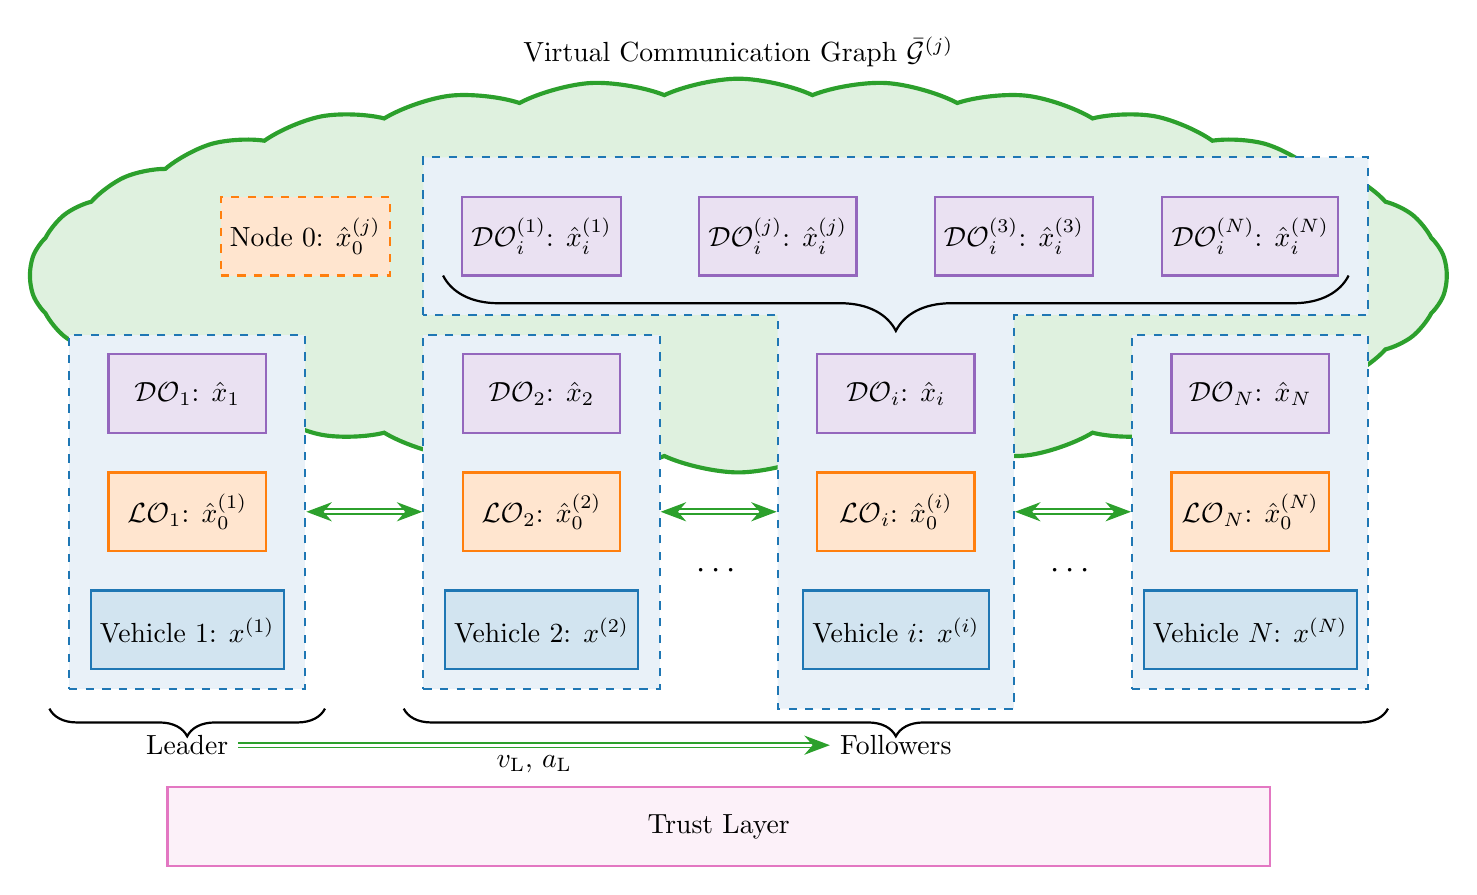
\begin{tikzpicture}[
    vehicle/.style={draw=blue1, fill=blue1!20, thick, minimum width=2cm, minimum height=1cm},
    localobs/.style={draw=orange1, fill=orange1!20, thick, minimum width=2cm, minimum height=1cm},
    distobs/.style={draw=purple1, fill=purple1!20, thick, minimum width=2cm, minimum height=1cm},
    sigarrow/.style={-stealth, thick, color=blue1},
    commarrow/.style={
    double,
    double distance=1pt,
    line width=0.7pt,
    draw=green1,
    {Stealth[scale=1.2]}-{Stealth[scale=1.2]}
    },
    physics/.style={draw=blue1, shape=rectangle, fill=blue1!10,line width=0.75pt,dashed,minimum width=3cm, minimum height=4.5cm}, %
    trust/.style={draw=rose1, shape=rectangle, fill=rose1!10,thick,minimum width=14cm, minimum height=1cm}
]
  %       		\draw [help lines,step=0.5cm] (0,0) grid (18,10); % 辅助网格 
		% % 画x和y轴坐标
		% \draw[stealth-,line width=2pt] (0,0)--(15,0);
		% % 画刻度
		% \foreach \x in {0,1,...,5}
		% {
		% 	\draw[xshift=\x cm] (0,0) -- (0,0.5);
		% };  
		% % 标坐标原点
		% \node[below] at (0,0){0};
		% %标x轴刻度值
		% \foreach \y in {1,2,...,18}
		% \node[below] at(\y,0){\y};

    \node[cloud,
            draw =green1,
            line width=1.5pt,
            text=cyan,
            cloud puffs = 30,
            cloud puff arc = 50,
            fill = green1!15,
            minimum width = 18cm,
            minimum height = 5cm,
            label=above:{Virtual Communication Graph $\bar{\G}^{(j)}$}
        ] (c) at(8.5, 4.5) {};
    
    \draw[draw=blue1,fill=blue1!10,dashed,line width=0.75pt] (4.5,4) -- (4.5,6)--(16.5,6) -- (16.5,4) -- (12,4) -- (12,-1) -- (9,-1) -- (9,4) -- (4.5,4) ;
    \draw [decorate, decoration={brace, mirror, amplitude=20pt}, thick]
    (4.75,4.5) -- (16.25,4.5);
    \draw [decorate, decoration={brace, mirror, amplitude=10pt}, thick]
    (4.25,-1) -- (16.75,-1)
    node[midway, below=6pt, name=followers] {Followers};
    \draw [decorate, decoration={brace, mirror, amplitude=10pt}, thick]
    (-0.25,-1) -- (3.25,-1)
    node[midway, below=6pt, name=leader] {Leader};
              
    \foreach \n in {1,2,3,4}
		{    
            \ifnum\n=3
                \node [name=PV\n,line width=0.75pt,minimum width=3cm, minimum height=4.5cm] at (4.5*\n-3,1.5) {};
            \else
                \node [physics,line width=0.75pt,name=PV\n] at (4.5*\n-3,1.5) {};
            \fi
            
            \ifnum\n=3
                \node[vehicle, name=V\n] at (4.5*\n-3, 0) {Vehicle $i$: $x^{(i)}$}; 
                \node[localobs,name=LO\n] at(4.5*\n-3,1.5) {$\LO_i$: $\hat{x}_{0}^{(i)}$};
                \node[distobs,name=DO\n] at(4.5*\n-3,3) {$\DO_i$: $\hat{x}_{i}$};
            \else
                \ifnum\n=4
                    \node[vehicle, name=V\n] at (4.5*\n-3, 0) {Vehicle $N$: $x^{(N)}$};
                    \node[localobs,name=LO\n] at(4.5*\n-3,1.5) {$\LO_N$: $\hat{x}_{0}^{(N)}$};
                    \node[distobs,name=DO\n] at(4.5*\n-3,3) {$\DO_N$: $\hat{x}_{N}$};
                \else
                    \node[vehicle, name=V\n] at (4.5*\n-3, 0) {Vehicle \n: $x^{(\n)}$}; 
                    \node[localobs,name=LO\n] at(4.5*\n-3,1.5) {$\LO_{\n}$: $\hat{x}_{0}^{(\n)}$};
                    \node[distobs,name=DO\n] at(4.5*\n-3,3) {$\DO_{\n}$: $\hat{x}_{\n}$};
                \fi
            \fi       
		};
    \foreach \j in {1,2,3,4}
    {
        \ifnum\j=2
                \node[distobs,name=DOi\j] at(3*\j+3,5) {$\DO_{i}^{(j)}$: $\hat{x}_{i}^{(j)}$};
            \else
                \ifnum\j=4
                    \node[distobs,name=DOi\j] at(3*\j+3,5) {$\DO_{i}^{(N)}$: $\hat{x}_{i}^{(N)}$};
                \else
                    \node[distobs,name=DOi\j] at(3*\j+3,5) {$\DO_{i}^{(\j)}$: $\hat{x}_{i}^{(\j)}$};
                \fi
            \fi
    
    };

    \node[localobs,name=node0,dashed] at(3,5) {Node 0: $\hat{x}_{0}^{(j)}$};
    \node[] at(8.25,0.75) {\large$\cdots$};
    \node[] at(12.75,0.75) {\large$\cdots$};

    \draw[commarrow,-{Stealth[scale=1.2]}] (leader) -- (followers) node[midway, below] {$v_{\text{L}}$, $a_{\text{L}}$};
    
    \draw[commarrow] (PV1) -- (PV2);
    \draw[commarrow] (PV2) -- (PV3);
    \draw[commarrow] (PV3) -- (PV4);

    \node[trust] at(8.25,-2.5) {Trust Layer};
    
    \end{tikzpicture}
    \caption{Schematic diagram of the estimation method.}
    \label{fig_observer_diagram}
\end{figure*}



\subsection{Main Objectives}

In previous work, the typical approach to designing a distributed observer relies on a known communication graph. In this context, the gain scale $w_{i l}$ is usually fixed. 
However, it is inevitable that cyber-attacks may occur, leading to changes in the communication graph.
To address the impact of the cyber-attack, we propose a synthetic framework that includes cyber-attack detection based on the concept of trust and the design of an online distributed observer. The trust is defined by the user based on estimations and measurements and will be used to determine how much the host vehicle trusts the data transferred from its neighbors. Based on this trust assessment, the observer gain will be updated to adapt to the new communication graph. Therefore, the main objectives of this paper can be summarized as follows:
\begin{itemize}
    \item Find a way to define the trust that can describe how much the host vehicle trusts the data transferred from its neighbors.
    \item Determine the updated law of gain scale $w_{i l}$ based on the trust and the gain matrix $F_{i}$ to make sure that~\eqref{eq_hatx_0} and~\eqref{eq_hatx_i} are satisfied simultaneously.
\end{itemize}



\section{Trust Score Framework}\label{sec_trust_score}
% Consider the cyber-attack, since the host vehicle cannot judge the value of a single data point received in a beacon, it has to be compared to the sender's actual behavior over a {\color{red}longer period of time.} 
% This allows the host vehicle to gain trust in the sender's benignity or detect misbehavior. 
% Depending on the trust in the predecessor and follower within the platoon, the host vehicle can regulate the safety gap to that vehicle. 
% If the trust falls below a certain threshold, it might ultimately decide not to be in a platoon with that vehicle at all. 
% This section introduces the details of trust, our trust-based misbehavior detection system for platoons. 

% \subsection{Description of the trust} 

According to the diagram of the estimation as shown in~Fig.~\ref{fig_observer_diagram} and the observer shown in~\eqref{eq_observer}, each distributed observer, denoted as $\DO_{i}^{(j)}$, receives two types of external information from its neighbors. The first type comes from other distributed observers, specifically $\DO_{l}^{(j)}$, where $\forall l \in {\N}_{i}$. The second type is derived from the local observer $\LO_{j}$. Our goal in assessing trust is to determine how much the distributed observer $\DO_{i}^{(j)}$ trusts these external signals by analyzing the information it receives.

To describe the trust framework, we designate a host vehicle $i$ and a target vehicle $l$  within the trust layer. The host vehicle will assess its level of trust in the target vehicle. The overall structure of this trust framework is illustrated in Fig.~\ref{fig_trust_framework}. In this context, we will define the following types of trust:
\begin{itemize}
    \item \textbf{Local Trust $\LT_{i,l}$}: The host vehicle $i$ evaluates the trust score for each local observer $\LO_{l}$ to form an opinion about the signal $\hat{x}_{0}^{(l)}$, where $l \in \N_{i}$, which is defined as \textit{Local Trust} $\LT_{i,l}$.
    \item \textbf{Global Trust $\DT_{i,l}$}: The host vehicle $i$ can evaluate the trust score for each distributed observer $\DO_{i}^{(l)}$ to obtain the opinion regarding the signal $\hat{x}_{l}$, where $l \in \N_{i}$. This is defined as \textit{Distributed Trust} $\DT_{i,l}$.
    \item \textbf{Target Trust $\T_{i,l}$}: Combining the Local Trust and Global Trust,  the host vehicle $i$ can evaluate the trust score for each target vehicle. This is defined as \textit{Distributed Trust} $\T_{i,l}$.
    \item \textbf{Vehicle Trust $\VT_{i}$}: Each vehicle $i$ has the trust score call \textit{Vehicle Trust} $\VT_{i}$ to gather the \textit{Local Trust} $\LT_{i,l}$ and \textit{Distributed Trust} $\DT_{i,l}$. 
\end{itemize}

\begin{figure*}[h!]

    \centering
    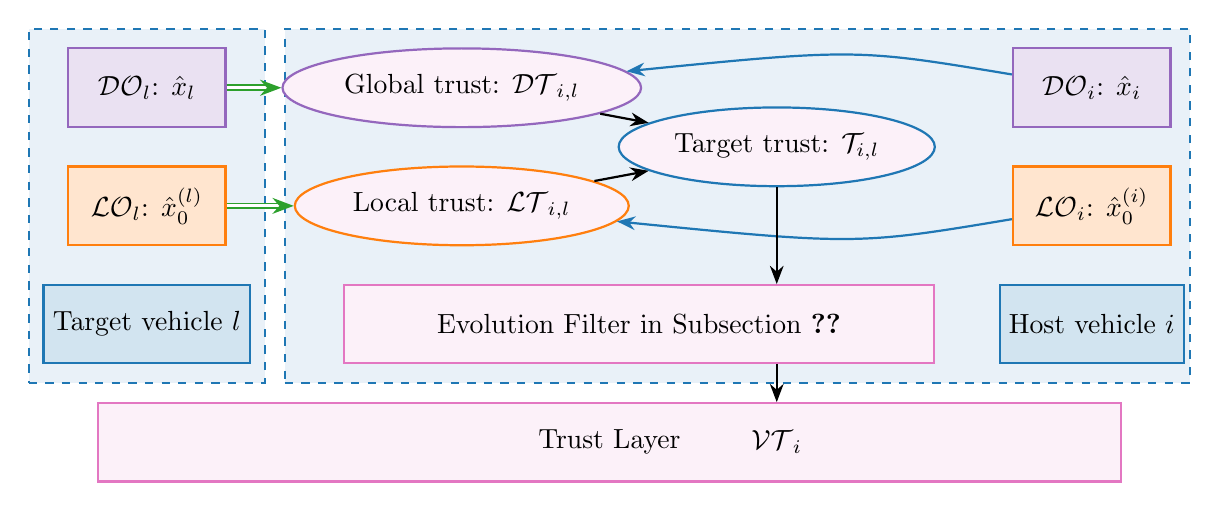
\begin{tikzpicture}[
    vehicle/.style={draw=blue1, fill=blue1!20, thick, minimum width=2cm, minimum height=1cm},
    localobs/.style={draw=orange1, fill=orange1!20, thick, minimum width=2cm, minimum height=1cm},
    distobs/.style={draw=purple1, fill=purple1!20, thick, minimum width=2cm, minimum height=1cm},
    sigarrow/.style={-Stealth, thick, color=blue1},
    commarrow/.style={
    double,
    double distance=1pt,
    line width=0.7pt,
    draw=green1,
    -Stealth
    },
    physics/.style={draw=blue1, shape=rectangle, fill=blue1!10,line width=0.75pt,dashed,minimum width=3cm, minimum height=4.5cm}, %
    trustlayer/.style={draw=rose1, shape=rectangle, fill=rose1!10,thick,minimum width=13cm, minimum height=1cm},
    trust/.style={draw=rose1, shape=ellipse, fill=rose1!10,thick,minimum width=1.5cm, minimum height=1cm}
]

  %     		\draw [help lines,step=0.5cm] (0,0) grid (18,10); % 辅助网格 
		% % 画x和y轴坐标
		% \draw[stealth-,line width=2pt] (0,0)--(15,0);
		% % 画刻度
		% \foreach \x in {0,1,...,5}
		% {
		% 	\draw[xshift=\x cm] (0,0) -- (0,0.5);
		% };  
		% % 标坐标原点
		% \node[below] at (0,0){0};
		% %标x轴刻度值
		% \foreach \y in {1,2,...,18}
		% \node[below] at(\y,0){\y};

        \node[physics,line width=0.75pt,minimum width=3cm, minimum height=4.5cm] at(2,1.5) { };
        \node[vehicle, name=target] at(2,0) {Target vehicle $l$};
        \node[localobs, name=LOt] at(2,1.5) {$\LO_{l}$: $\hat{x}_{0}^{(l)}$};
        \node[distobs, name=DOt] at(2,3) {$\DO_{l}$: $\hat{x}_{l}$};

        \node[physics,line width=0.75pt,minimum width=11.5cm, minimum height=4.5cm,name=host] at(9.5,1.5) {};
        \node[vehicle,name=host] at(14,0) {Host vehicle $i$};
        \node[localobs,name=LOh] at(14,1.5) {$\LO_{i}$: $\hat{x}_{0}^{(i)}$};
        \node[distobs,name=DOh] at(14,3) {$\DO_{i}$: $\hat{x}_{i}$};
        

        \node[trust,draw = purple1, name=DT] at(6,3) {Global trust: $\DT_{i,l}$};
        \node[trust,draw = orange1, name=LT] at(6,1.5) {Local trust:  $\LT_{i,l}$};
        \node[trust,draw = blue1, name=T] at(10,2.25) {Target trust: $\T_{i,l}$};
        % \node[trust] at(10,0) {$\VT_{i}$};

        \node[trust,shape=rectangle,name=evo, minimum width=7.5cm] at(8.25,0) {Evolution Filter in Subsection~\ref{sec_Evolution_trust} }; 
        \node[name=evo,minimum height=1cm] at(10,0) {};

        \node[trustlayer] at(0.5/2+15.25/2,-1.5) {Trust Layer};
        \node[name = VT,minimum height=1cm] at(10,-1.5) {$\VT_{i}$};
    
        \draw[commarrow] (DOt) -- (DT);
        \draw[commarrow] (LOt) -- (LT);

        \draw[sigarrow] (LOh) .. controls +(-3,-0.5).. (LT);
        \draw[sigarrow] (DOh) .. controls +(-3,0.5).. (DT);

        \draw[sigarrow, black] (LT) -- (T);
        \draw[sigarrow,black] (DT) -- (T);

        \draw[sigarrow,black] (T) -- (evo);
        \draw[sigarrow,black] (evo) -- (VT);

        
        
    \end{tikzpicture}
    \caption{Trust framework.}
    \label{fig_trust_framework}
\end{figure*}


In the following subsections, we will explain how to calculate the trust. After that, we will provide more details on how to determine vehicle trust ($\VT_{i}$) and how to utilize it effectively.

\subsection{Local Trust}
\label{sub:local_trust}
% We assume that the host vehicle with automated driving functions must ultimately trust its sensor data. 
% When assessing other vehicles' trustworthiness, the host vehicle uses its sensor data as ground truth to compare the others' actual behavior to what they announced in their beacons. 
% This comparison is feasible only for vehicles within the perception range of the host vehicle's local sensors and is most effective for the direct predecessor and successor. 

In the context of the local trust, we will focus on the host vehicle $i$. We define the target vehicle $l$ is the neighbor of the host vehicle, which means $l \in {\N}_{i}$. And $\LT_{i,l}$ represents how the host vehicle trusts the target vehicle $l$. 
To clarify, we give the final result of $\LT_{i,l}$ as
\begin{equation}
    \LT_{i,l}= \iota_{i,l}^\text{time} \cdot (\iota_{i,l}^\text{velocity})^\mathbf{v} \cdot (\iota_{i,l}^\text{distance})^\mathbf{d} \cdot (\iota_{i,l}^{\text{accel}})^\mathbf{a}
\end{equation}
where $\iota_{i,l}^\text{velocity}, \iota_{i,l}^\text{distance}, \iota_{i,l}^\text{accel}, \iota_{i,l}^\text{time}$ represents the different components of the local trust, which will be explained in the following sections. The exponential weight $\mathbf{v},\mathbf{a},\mathbf{d}$ controls how sensitive each component is to local trust. 

\subsubsection{Velocity}
The host vehicle $i$ calculates the reference velocity $v_{\text{ref}}(t)$ based on the leader's velocity $v_{\text{L}}(t-b_{\text{L}})$, adjusted by the estimated acceleration $a_{\text{L}}(t-b_{\text{L}})$ and the elapsed time $t_{\text{elap}}$ since the last send leader beacon :
\begin{equation}
    v_{\text{ref}}(t) = {v}_{\text{L}}(t-t_{\text{elap}}) + t_{\text{elap}} \cdot {a}_{\text{L}}(t-t_{\text{elap}}), 
\end{equation}

% For the target vehicle $j$, where $j \in \bar{\N}_{i}^{(j)}$
Then, the mismatch score of the target vehicle $i$ with the leader, can be calculate as
\begin{equation}
    v_{l,\text{L}} = 
        \begin{cases} 
            \max\left(1 - \left|\dfrac{\hat{v}_{0}^{(l)} - v_{\text{ref}}}{v_{\text{ref}}}\right|,\  0\right), & \text{if } v_\text{ref} > 0, \\
            \max\left(1 - | \hat{v}_{0}^{(l)}|,\  0\right), & \text{otherwise},
        \end{cases}
\end{equation}
where the subscript L means "Leader". 
$v_{l,\text{L}}$ denotes how well the estimated velocity $\hat{v}_{0}^{(l)}$ from the local observer $\LO_{l}$ matches the leader's velocity. 

Similarly, to reflect the the divergence between the local estimated velocity from the host vehicle and its neighbors, the following mismatch score is proposed
\begin{equation}
    v_{l,\text{H}} = 
        \begin{cases} 
            \max\left(1 - \left|\dfrac{\hat{v}_{0}^{(l)} - \hat{v}_{0}^{(i)}}{\hat{v}_{0}^{(i)}}\right|,  0\right), & \text{if} \  \hat{v}_{0}^{(i)} > 0, \\
            \max\left(1 - |\hat{v}_{0}^{(l)}|,  0\right), & \text{otherwise},
        \end{cases}
\end{equation}
where the subscript "H" means "Host". 



Fusion of these mismatches using a weighted average:
\begin{equation}
    \iota_{i,l}^\text{velocity} = ((1-\sigma) v_{l,\text{L}} +\sigma  v_{l,\text{H}})    
\end{equation}
where $\sigma$ is the weighted scale, which can be chosen depending on the index position of the target vehicle $l$. If the target is following the host vehicle $i$, then $\sigma$ will ideally be around 0-0.3. If the target is ahead of the host, $\sigma$ will be around 0.7-1.


\subsubsection{Distance}
The host vehicle $i$ calculates the distance with respect to the target $l$ according to the following 
% \begin{equation*}
%     d_{i,l} = \sqrt{(\hat{s}_{\text{x,}0}^{(l)} - \hat{s}_{\text{x,}0}^{(i)})^2 + (\hat{s}_{\text{y,}0}^{(l)} - \hat{s}_{\text{y,}0}^{(i)})^2} - L,
% \end{equation*} 

\begin{equation*}
    d_{i,l} = \hat{s}_{\text{x,}0}^{(l)} - \hat{s}_{\text{x,}0}^{(i)} - L,
\end{equation*} 

where $L$ is the length of the vehicle. 
So the mismatch between the measured distance $d$ from its sensors and the calculated data $d_{k,i}$ is 
\begin{equation}
    \iota_{i,l}^{\text{distance}} = \max\left(1 - \left|\frac{d_{i,l} - d}{d}\right|, 0\right).
\end{equation}

\begin{assumption}
    When the vehicle is connected, it knows basic information about its neighbors, such as the type and length of the vehicle.
\end{assumption}
% \begin{remark}
%     If the target vehicle is neither in front of nor behind the host vehicle, we can adjust the weight of the distance score. Since we don't have exact measurements for this case, we will use a generally accepted expected distance instead. That defines by the controller in Section \ref{sec_simulation}
% \end{remark}

\subsubsection{Acceleration}
The host vehicle can calculate the expected relative acceleration as 
\begin{equation}
    % v_\text{rel} = \dfrac{d(t-1) - d(t)}{t_s},
    a_{rel}^{expect} = \dfrac{v_{rel}(t) - v_{rel}(t-n) }{n},
    % a_{rel}^{recv} = \hat{a}_0^{(l)} - \hat{a}_0^{(i)}
\end{equation}
 which is derived as the rate of change in relative velocity $v_{rel}$ over the interval $n$, where $ n$ is chosen to avoid noise.
The relative acceleration according to recveicd data of target l is 
\begin{equation}
a_{rel}^{recv} = \hat{a}_0^{(l)} - \hat{a}_0^{(i)}
\end{equation}
Define regulation constant $C$ and distance adjustment $d_{\text{adj}}$:
\begin{equation}
d_{\text{add}} = \frac{d_{\text{norm}} \cdot |\text{Idx}_{\text{target}} - \text{Idx}_{\text{host}}|}{d}    
\end{equation}
where $Idx$ is the position index of the vehicle in the platoon, $d_{\text{norm}}$ is a safe threshold distance that depends on the controller's maximum distance between two consecutive vehicles, more details in the Section \ref{sec_simulation}. 
% If $\text{ID}_{\text{target}} > 1$:
%       $$
%       \text{SignMismatch} = \begin{cases}
%       0 & \text{if } \text{sign}(a_{\text{host}}) = \text{sign}(a_{\text{rel,actual}}) \\
%       1 & \text{otherwise}
%       \end{cases}
%       $$
%       $$
%       C = \begin{cases}
%       0.8 & \text{if SignMismatch} = 0 \\
%       0.85 & \text{if SignMismatch} = 1
%       \end{cases}
%       $$

%     $$
%     d_{\text{add}} = \frac{d_{\text{norm}} \cdot C}{d_k}
%     $$
% Else (i.e., $\text{ID}_{\text{target}} \leq 1$):

% $$
% d_{\text{add}} = \frac{d_{\text{norm}} \cdot C}{d_k} \quad \text{(with default } C = 1 \text{)}
% $$

Then the trust score of the acceleration of the target is 
\begin{equation}
   \iota_{i,l}^{\text{accel}} = \max\left(1 - \left| d_{\text{adj}} \cdot \left(a_{rel}^{recv} - a_{rel}^{expect}  \right) \right|, 0\right)
\end{equation}
where $\left(a_{rel}^{recv} - a_{rel}^{expect}  \right)$ is the difference of relative acceleration between the neighbors of the host and itself.  
The term $d_{\text{adj}}$ scales mismatch based on the distance between the 2 vehicles 
% how fast the vehicles are moving relative to each other.

Acceleration differences matter more if two vehicles are close together and moving at different speeds.
If they are farther apart or moving at the same speed, acceleration differences are less critical.
% This prevents small acceleration mismatches from being overly penalized when relative motion is low.

\subsubsection{Data Delivery Timeout}
\begin{equation}\label{deli_timeout}
    \iota_{i,l}^{\text{time}} =\begin{cases}
        0 , &\text{No beacon data is received,} \\
        1, &\text{otherwise.}\\
    \end{cases}
\end{equation}
where $\iota_{i,l}^{\text{time}}$ indicates whether host vehicle $l$ sends a local beacon data on time to vehicle $i$. A value of 0 means the beacon was not received in time (possible loss or delay), while 1 means it was received as expected.






% \subsubsection{Heading Angle}
% The direction of motion represents the target's estimated heading. This can be calculated using the arctangent function:
% \begin{equation}
%     \theta_{\text{est}} = \arctan \left(\hat{s}_{\text{y},0}^{(l)}(t) - \hat{s}_{\text{y},0}^{(l)}(t-1), \hat{s}_{\text{x},0}^{(l)}(t)- \hat{s}_{\text{x},0}^{(l)}(t-1)  \right).   
% \end{equation}
% Compared with the reported heading from the host vehicle, $\hat{\theta}_{0}^{(i)}$, the difference of the heading between the target and the host is 
%  \begin{equation}
%     \theta_{\text{diff}} = \min \left(|\hat{\theta}_{0}^{(i)}- \theta_{\text{est}}|, 2\pi - |\hat{\theta}_{0}^{(i)} - \theta_{\text{est}}| \right),
% \end{equation}
% which ensures the smallest angle difference is used, considering that the headings are circular from $0$ to $2\pi$.
% A trust value for the heading can be defined, decreasing as the difference grows:
% \begin{equation}
%     \iota_{i , l}^{\text{angle}} = \max\left(1 - \frac{\theta_{\text{diff}}}{\theta_{\text{max}}}, 0\right). 
% \end{equation}
% Here, $\theta_{\text{max}}$ is a threshold (e.g.,$\pi/10$ radians). If $\theta_{\text{diff}}$ exceeds $\theta_{\text{max}},$ the trust drops to zero, indicating unreliable heading data.

% when evaluating the trust for local data


\subsection{Global Trust}
In the context of the global trust, we will focus on the host vehicle $i$. The target vehicle $l$ should be $l \in \N_{i}$. And $\DT_{i,l}$ represents how the host vehicle $i$ trusts the global estimation from target vehicle $l$, which is defined as
\begin{equation}
\DT_{i,l} =  \gamma_{i,l}^{\text{time}} \cdot  \gamma_{i,l}^{\text{host}} \cdot \gamma_{i,l}^{\text{local}}, 
\end{equation}
where $\gamma_{i,l}^{\text{time}}$ is same in \eqref{deli_timeout} , $\gamma_{l}^{\text{host}}$ and $\gamma_{i,l}^{\text{local}}$ are applied to check if the global estimates from neighbor $l$ are consistent with the host's and the local measurements, respectively; 
Both of them will be illustrated in the following. 

\subsubsection{Consistency with host's global estimate}
To assess whether the global estimate from the target $l$ is trustworthy, the host can compare it directly to its own global estimate. We use the \textbf{Mahalanobis distance}, which normalizes discrepancies based on covariance:
\begin{equation}
    d_{i,l}^{(j)} = \left( \hat{x}_i^{(j)} - \hat{x}_l^{(j)} \right)^{\top} \Sigma_{\text{host}}^{-1} \left( \hat{x}_i^{(j)} - \hat{x}_l^{(j)} \right), 
    \label{eq_dis_glo}
\end{equation}
where $\Sigma_{\text{local}}$ is the diagonal covariance matrix  which captures variance and correlations between state variables defined as 
\begin{equation}
\Sigma_{\text{local}} = \diag{\sigma^2_1, \sigma^2_2, \cdots , \sigma^2_n},
\end{equation}
where $n$ is the number of states in the vehicle, and $\sigma^2_k$ is  the variance of discrepancies about the different states. 

And then, add up these differences to get the total discrepancy score across the platoon as the following
\begin{equation}
    D_{i,l} = \sum_{j=1}^N d_{i,l}^{(j)}.
\end{equation}
A small  $D_{i,l}$ means the global estimate from vehicle $l$ is close to the host's, suggesting higher trustworthiness.

Based on the total discrepancy score across the platoon, the trust score can be converted to be 
\begin{equation}
    \gamma_{i,l}^{\text{host}} = \exp\left( -{D_{i,l}} \right).
\end{equation}
The result,  $\gamma_{i,l}^{\text{host}}$, ranges from 0 to 1. A value near 1 means high trust (small discrepancy), while a value near 0 means low trust (large discrepancy).

\begin{remark}[Explanation on $\Sigma_{\text{local}}$]
If the variance of an element's state (such as position, velocity, or acceleration) is high, then \( \sigma^2_n \) will also be large. This means that discrepancies in that element will contribute less to the overall score. Conversely, if the variance is low, the discrepancies will have a greater impact on the score.
% \begin{itemize}
%     \item If velocity has high variance, \( \sigma^2_v \) will be large, making velocity discrepancies contribute less to the final distance.
%     \item If position has low variance, \( \sigma^2_p \) will be small, making position discrepancies contribute more.
%     % \item If acceleration and velocity are correlated, Mahalanobis distance accounts for this, \( \mathbf{\Sigma} \) will contains off-diagonal terms capturing dependencies.
% \end{itemize}
\end{remark}

\subsubsection{Consistency with host's local measurement}
Host vehicle  $i$  uses its sensors to measure the relative state of nearby vehicles (e.g., distance and relative velocity to a predecessor and a follower) and checks if the global estimates from neighbor  $l$  are consistent with these measurements.

Let $y_{i,j}(t)$ be vehicle  $i$ 's sensor measurement of vehicle $ j $'s state relative to itself (e.g., $ y_{i,j}(t) = x^{(j)}(t) - x^{(i)}(t) $ for relative position). This is available for vehicles $ j \in \N_i$. 

For neighbor $l$ 's global estimate to be plausible, it should satisfy expectively:
\begin{equation*}
    \hat{x}_l^{(j)}(t) - \hat{x}_l^{(i)}(t) \approx y_{i,j}(t).
\end{equation*}

Define the error between the global estimate and the local measurement as
\begin{equation}
    \varepsilon_{i,l}^{(j)}(t) = \left( \hat{x}_l^{(j)}(t) - \hat{x}_l^{(i)}(t) \right) - y_{i,j}(t), 
\end{equation}
Similar with the \eqref{eq_dis_glo}, by applying the covariance matrix $\Sigma_{\text{local}}$, we can get 
\begin{equation}
    \varepsilon_{i,l}^{(j)}(t) = (\varepsilon_{i,l}^{(j)}(t))^{-1} \Sigma_{\text{local}}^{-1} \varepsilon_{i,l}^{(j)}(t).
\end{equation}

Then, the total consistency error can be get by summing up the errors over all measurable vehicles:
\begin{equation} 
    E_{i,l}(t) = \sum_{j \in \N_i} E_{i,l}^{(j)}(t).
\end{equation}
A higher $E_{i,l}(t)$  suggests that neighbor  $l$ 's global estimate contradicts local sensor data.

Convert the error into a trust factor as
\begin{equation}
    \gamma_{i,l}^{\text{local}}(t) = \exp\left( -{E_{i,l}(t)} \right),
\end{equation}
where $\gamma_{i,l}^{\text{local}}(t) \in (0, 1]$, with lower values indicating poor consistency. 


\subsection{The Single Trust of the Target at step $t$}  
We can combine the global trust and the local trust to get the final trust of the target $l$ in opinion from the host vehicle $i$, which is shown in 
\begin{equation}
    \T_{i,l}(t) =  \LT_{i,l} \cdot \DT_{i,l}. 
    \label{trs_sample_genral}
\end{equation}

Now, $\T_{i,l}(t)$ is the single trust score indicates the quality of target $l$'s data at the time $t$.

\begin{remark}
    While we will proceed with trust, we must not forget the importance of prior calculations. This means we can flag anomalies when something appears to be incorrect. For instance, in the calculation of global trust, we consider the local gamma and cross gamma. 
    If either of these values is abnormally low, we will raise a flag to the use after.
\end{remark}

\subsection{Building Evolution Trust of the Target} \label{sec_Evolution_trust}
To capture the evolution of trust of the target vehicle over time, the trust $\T_{i,l}(t)$ is formed through continuous observation and repeated interactions. 
Therefore, the trust samples obtained-denoted as in \eqref{trs_sample_genral} must be aggregated in a manner that reflects both historical progression and the associated uncertainty or confidence in the assessment. 
This motivates the use of probabilistic modeling, particularly through Bayesian statistical frameworks. 

In this study, we define a five-level trust quality rating scale $q = 5$, consisting of mutually exclusive and equidistant categories: \textit{untrustworthy}, \textit{bad}, \textit{acceptable}, \textit{good}, and \textit{excellent}, spanning the interval $[0, 1]$. When the host vehicle $i$ computes a trust value $\T_{i,l}(t) \in [0, 1]$ for a neighboring vehicle $l$, the result is discretized into a one-hot vector $r_{i,l}(t) \in \mathbb{R}^q$, where the position corresponding to the appropriate trust level is set to 1 and all others are 0, which means that for any $k = 1, \cdots q$, there is
\begin{equation}
    \text{e}_{q}^{\top}(k)r_{i,l} (t) = \begin{cases}
        1, & \text {the trust rank is $k$}, \\
        0 , & \text {otherwise},
    \end{cases}
\end{equation}
which represents a categorical trust sample with a single outcome. 

Over time, the accumulated trust vector $R_{i,l}(t)$ for target vehicle $l$ is updated using a weighted aggregation of past interactions: 
\begin{equation}
    R_{i,l}(t + 1) = \left(1 - \T_{i,l}(t) \cdot \beta \right) \cdot R_{i,l}(t) + r_{i,l}(t),
\end{equation}
where $\T_{i,l}(t)$ representing the current trust score and $\beta \in [0, 1]$ as a tunable weight that modulates trust adaptability. 
The term, $\T_{i,l}(t) \cdot \beta$, controls how quickly past experiences decay. 

The parameter $\beta$ governs the responsiveness of the trust model:
\begin{itemize}
    \item A higher $\beta$ (e.g., $0.7$-$0.8$) is applied during \textit{longitudinal behavior} scenarios, where misbehavior must be quickly reflected by a drop in trust.
    \item A lower $\beta$ (e.g., $0.4$-$0.6$) is used during \textit{lane changes}, where occasional irregularities may be misinterpreted as attacks. This helps mitigate \textit{false positives}, such as when a vehicle is mistakenly perceived as malicious due to legitimate but abrupt maneuvers.
\end{itemize}

Finally, at the current step $t$ (in the following, we omit $t$ for simplifying), a normalized trust distribution vector $S_{i,l}(k)$ is computed by incorporating an a priori distribution $\alpha$ and a confidence parameter $C$:
\begin{equation}
    S_{i,l}(k) = \dfrac{R_{i,l}(k) + C \cdot \alpha(k)}{C + \sum_{j=1}^{q} R_{i,l}(j)},
\end{equation}
which provides a probabilistic interpretation of the trustworthiness of the target vehicle $l$, blending historical observations with prior beliefs to produce a robust and adaptive trust estimate. 

The trust score $\VT_{i,l}$ is then calculated as:
\begin{equation}
    \VT_{i,l} = \sum_{j=1}^{q} \dfrac{j-1}{q-1} \cdot S_{i,l}(j).
\end{equation}
Now, the trust toward to the target, $\VT_{i,l}$, from the host has been obtained. In the following section, the general trust for all vehicles in the platoon will be presented.

\subsection{Building general trust for all vehicles}
We define a row vector $\O_{i} \in \mathbb{R}^{1 \times N}$ as the general trust for the platoon from the host vehicle $i$, whose element at the $l$-th index means the opinion of the target $l$ from the host vehicle $i$. Here, the definition of each element of  $\O_{i}$ is given as
\begin{equation}
    \O_{i}(j) = \begin{cases}
        1, & j = i,\\
        \VT_{i,j}, & j \in \N_{i},\\
        \dfrac{\O_{i,j}^{\text{dis}} +  \O_{i,j}^{\text{popa}} }{2}, & j \notin \{\N_{i} \cup  \{ i \}\}, 
    \end{cases} 
    \label{eq_VTi(j)}
\end{equation}
where $\O_{i,j}^{\text{dis}}$ is is based on the inverse distance and $\O_{i,j}^{\text{popa}}$ is  based on the trust propagation. Both of them are utilized to calculate the trust of vehicle $j$, where $j \notin \{\N_{i} \cup  \{ i \}\}$. 

According to \eqref{eq_VTi(j)}, when $j = i$, $\O_{i}(j)= 1$ means that each vehicle trust itself. For the neighbors of the vehicle, which means $j \in \N_{i}$, the trust is defined in the previous section. And for vehicle $j$ without communication to vehicle $j$, 
to avoid the identification mistake, we utilize trust of vehicle $j$ from other vehicles, to approximate it, which is known as opinion-based trust aggregation.  

For the inverse distance-based weighting function, $\O_{i,j}^{\text{dis}}$ is defined as
\begin{equation}
   \O_{i,j}^{\text{dis}} = \displaystyle \sum_{k \in \N_{j}  } \left( g_{i,k} \cdot \O_{k}(j) \right). 
\end{equation}
where 
\begin{equation}
    g_{i,k} = \dfrac{\bar{g}_{i,k}}{\sum_{k \in \{\N_{j} \}  } \bar{g}_{i,k}}, \quad \bar{g}_{i,k} = \dfrac{1}{1 + |i - k|},
\end{equation}
where $|t - j|$ is the index distance of the vehicle $i$ and $k$ in the platoon. 
This weight ${g}_{i,k}$ ensures that closer vehicles are more important. 

Considering the trust propagation, $\O_{i,j}^{\text{popa}}$ is
\begin{equation}
   \O_{i,j}^{\text{popa}} = \dfrac{\displaystyle \prod_{p=i}^{j+1} \O_p(p-1) + \displaystyle \prod_{p=i}^{j-1} \O_p(p+1)}{2},
\end{equation}
where $\displaystyle \prod_{p=i}^{j+1} \O_p(p-1)$ is for $i > j$, and $\displaystyle \prod_{p=i}^{j-1}$ is for $i < j$.

\begin{remark}[Explanation to inverse distance]
After calculating $\O_{i}(j)$ under the case $j=1$ and $j \in \N_{i}$ for all $i \in \V$, Fig.~\ref{fig_VT_distance} shows how to calculate $\O_{i}(j)$ for $j \notin \{\N_{i} \cup  \{ i \}\}$, which is presented as $*$. 
\begin{figure}
    \centering       
    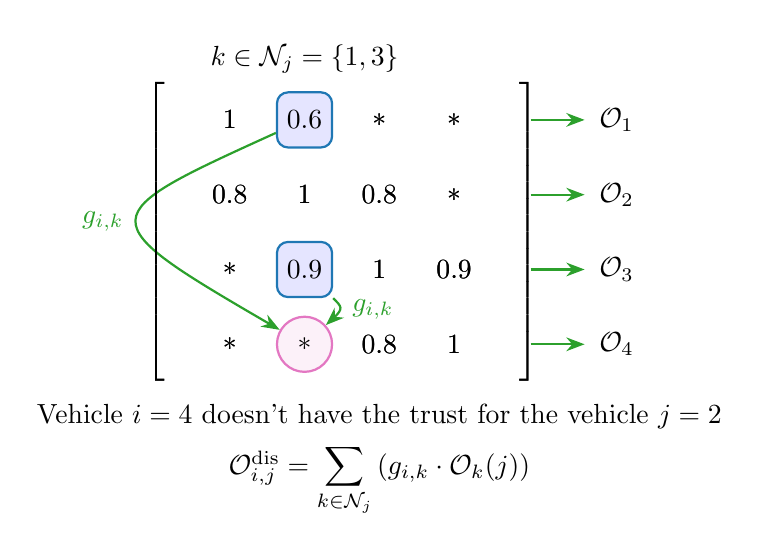
\begin{tikzpicture}[
    every node/.style={minimum size=8mm, anchor=center},
    myarrow/.style={-Stealth, thick, green1},
    highlight/.style={circle, draw=rose1,  fill = rose1!10, thick},
    colframe/.style={rectangle,draw=blue1, fill = blue!10, thick, rounded corners}
]
% Matrix with placeholders
\matrix (m) [matrix of math nodes, 
nodes in empty cells, 
left delimiter={[}, right delimiter={]}, row sep=0.15cm, 
column sep=0.15cm
] {
    1 & 0.6 & * & * \\
    0.8 & 1 & 0.8 & * \\
    * & 0.9 & 1 & 0.9 \\
    * & * & 0.8 & 1 \\
};

% Draw arrows for row names
\foreach \i in {1,...,4} {
    \node[right=1.25cm of m-\i-4] (r\i) {$\O_{\i}$};
    \node[right=-0.25cm of m-\i-4] (b\i) {};
    \draw[myarrow] (b\i) -- (r\i);
}

% Highlight the element at (4,2)
\node[highlight, minimum size=7mm, name=m42] at (m-4-2) {};
\node [below=0.1cm of m-4-3] (text) {Vehicle $i=4$ doesn't have the trust for the vehicle $j=2$};
\node [below=0.75cm of m-4-3] (eq) {$\O_{i,j}^{\text{dis}} = \displaystyle \sum_{k \in \N_{j}  } \left( g_{i,k} \cdot \O_{k}(j) \right)$};

% Rectangle around 2nd column except (2,2)
\node[colframe, minimum size=7mm, name=m12, label=above:{$k \in \N_{j} = \{1,3\}$}] at (m-1-2) {};
\node[colframe, minimum size=7mm,name=m32] at (m-3-2) {};

\draw[myarrow] (m12) .. controls +(-2.75,-1.25) .. node[midway,left] {$g_{i,k}$}(m42);
\draw[myarrow] (m32) .. controls +(0.5,-0.5) .. node[midway,right] {$g_{i,k}$}(m42);

\matrix (m2) [matrix of math nodes, 
nodes in empty cells, 
left delimiter={[}, right delimiter={]}, row sep=0.15cm, 
column sep=0.15cm
] {
    1 & 0.6 & * & * \\
    0.8 & 1 & 0.8 & * \\
    * & 0.9 & 1 & 0.9 \\
    * & * & 0.8 & 1 \\
};

\end{tikzpicture}
    \caption{Weight based distance for $\O_{i,j}^{\text{dis}} $.}
    \label{fig_VT_distance}
\end{figure}
    
\end{remark}

\begin{remark}[Explanation to the trust propagation]
After calculating $\O_{i}(j)$ under the case $j=1$ and $j \in \N_{i}$ for all $i \in \V$, we can get the trust graph $\G_{\text{T}} = \{ \V,\ \E,\ \mathcal{W}_{\text{T}}\}$, where $\mathcal{W}_{\text{T}}$ is the trust between each node, which is shown in Fig.~\ref{fig_VT_popa}. Here, $\O_{i,j}^{\text{popa}}$ is calculated by multiple products all the trust on the path from node $i$ to node $j$. 

\begin{figure}
    \centering       
    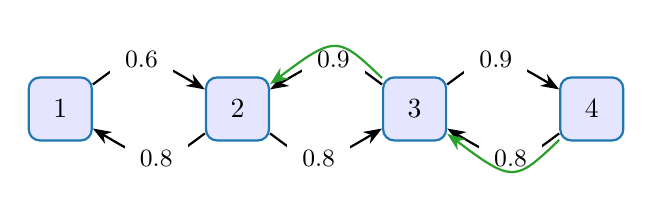
\begin{tikzpicture}[
    every node/.style={minimum size=8mm, anchor=center},
    myarrow/.style={-Stealth, thick, black},
    highlight/.style={circle, draw=rose1,  fill = rose1!10, thick},
    colframe/.style={rectangle,draw=blue1, fill = blue!10, thick, rounded corners}
]


% Draw arrows for row names
\foreach \i in {1,...,4} {
    \node[colframe,name=node\i] at(2.25*\i,0) {$\i$};
}
\draw[myarrow] (node1) .. controls +(1,0.75) .. node[midway,fill=white] {\small$0.6$}(node2);

\draw[myarrow] (node2) .. controls +(-1,-0.75) .. node[midway,fill=white] {\small$0.8$}(node1);
\draw[myarrow] (node2) .. controls +(1,-0.75) .. node[midway,fill=white] {\small$0.8$}(node3);

\draw[myarrow] (node3) .. controls +(-1,0.75) .. node[midway,fill=white] {\small$0.9$}(node2);
\draw[myarrow] (node3) .. controls +(1,0.75) .. node[midway,fill=white] {\small$0.9$}(node4);

\draw[myarrow] (node4) .. controls +(-1,-0.75) .. node[midway,fill=white] {\small$0.8$}(node3);


% \draw[myarrow, color=green1] 
%   (node4) .. controls +(-1,-0.85) and +(1,0.85) .. (node2);

  \draw[myarrow, color=green1] 
  (node4) .. controls +(-1,-0.95) .. (node3);
   \draw[myarrow, color=green1] 
  (node3) .. controls +(-1,0.95) .. (node2);


\end{tikzpicture}
    \caption{Weight based distance for $\O_{i,j}^{\text{popa}} $.}
    \label{fig_VT_popa}
\end{figure}

\end{remark}

\section{Weight Design for observer based on the trust}\label{sec_Weigth_Design}
In this section, based on the trust information, we provide a simple strategy to identify which vehicle is legitimate and which is malicious. Then according to the number of legitimate neighbors, the observer gains $w_{il}^{j}(t)$ will be given.

\subsection{Weight based on the trust}
First, we redefine a time-dependent set of legitimate neighbors for each vehicle $i$ under the virtual communication graph $\bar{\G}^{{(j)}}$ as
\begin{equation}
\mathcal{LN}_i^{(j)}(t)= 
\begin{cases}
    \left\{l \in \V| \  \O_{i}(l) > 0.5 \right\} \cup \left\{0 \right\},  & \text{if}\  \O_{i}(j)>0.5, \\
    \left\{l \in \V| \  \O_{i}(l) > 0.5 \right\}, & \text{if}\  \O_{i}(j) \leq 0.5,
\end{cases}
\end{equation}
where the set, $\left\{l \in \V| \  \O_{i}(l) > 0.5 \right\}$, is the  legitimate neighbors under the real graph $\G$. Because we add the local observer $\LO_{j}$ as the virtual node $0$ in the virtual communication graph $\bar{\G}^{{(j)}}$,  this virtual node $0$ also should be considered. If the host vehicle $i$ has a good opinion of the vehicle $j$, it means that the node $0$ also is legitimate neighbors.  

Denote the following 
\begin{equation}\label{new_setneibor}
n_{il}^{(j)}(t)=\max \left\{\kappa,\left|\mathcal{LN}_i^{(j)}(t)\right|+1\right\} \geq 1 \quad \text { for all } l \in \mathcal{LN}_i^{(j)}.
\end{equation}
where $\kappa >0$ is the parameter to limit the maximum influence from the neighbors of $i$th vehicle. 
Then, the observer's weight gain can be chosen as
\begin{equation}\label{design_gain}
    w_{il}^{(j)}(t) = \begin{cases}
        \dfrac{1}{n_{il}^{(j)}(t)}, & l \in \mathcal{LN}_i^{(j)}(t)\\
        0 ,& \text{otherwise}.
    \end{cases}
\end{equation}

For a more robust design, we want further to design the weight gain $w_{i0}^{(j)}(t)$ in \eqref{eq_observer} based on the local trust of the target vehicle $l$ from the host vehicle $i$ that we are calculated in \ref{sub:local_trust}.
\begin{equation}\label{redesign_gain_virtual}
    w_{i0}^{(j)}(t) = \begin{cases}
        \dfrac{1}{n_{il}^{(j)}(t)}, & \LT_j > 0.5\\
        0 ,& \text{otherwise}.
    \end{cases}
\end{equation}



According to the weight gain, the communication graph will be switched depending on the time. To ensure the connectivity of the communication graph, we list the following assumptions.


\begin{assumption}[Jointly connected graph \cite{hao2024eventtriggered,liu2021discretetime}]
\label{ass_graph}
A switching-directed graph is said to be jointly connected if there exists a positive constant $T > 0$ such that the union of the subgraphs over $[t, t+ T]$, $\forall t \geq 0$ that is, $\cup _{[t, t+ T]}\bar{\G}^{(j)}(t)$, contains a spanning tree.
\end{assumption}

% \textcolor{red}{Huy: I put the proof here, so we can have 2 subsection: Proof for normal case, and proof for attack case when we apply our observer Weigth ~\eqref{Weigth_Design} }

\subsection{Stability of the error }
\label{subsec_Prove}

In this subsection, we explore the conditions that guarantee the stability of the
estimation error dynamics of the proposed observer, as given in~\eqref{eq_observer}.

For the estimation error of the vehicle $j$ from the local observer $\LO_{j}$, we denote
\begin{equation}
    e_0^{(j)}(t) = \hat{x}_0^{(j)}(t) - x^{(j)}(t), \quad j \in \V. 
\end{equation}
Similarly, for the estimation error of the vehicle $j$ from the distributed observer $\DO_{i}^{(j)}$, we denote
\begin{equation}
    e_i^{(j)}(t) = \hat{x}_i^{(j)}(t) - x^{(j)}(t), \quad j \in \V, \ i \in {\V}.
\end{equation}

Then, estimation error of the $j^{th}$ vehicle state estimated by the observer implemented on vehicle $i$ is defined as: 
\begin{equation}
\begin{cases}
    \begin{aligned}
        e_0^{(j)}(t+1) =& \left( A_{\text{b}} - F_{j} C_{\text{b}}  \right) e_0^{(j)}(t), \\
        e_i^{(j)}(t+1) =& A_{\text{b}}\left[e_i^{(j)}(t) + \sum_{l \in \mathcal{N}_i} w_{il}^{(j)} (e_l^{(j)}(t) - e_i^{(j)}(t))\right. \notag \\
    &+\left.  w_{i0}^{(j)}(e_0^{(j)}(t) - e_i^{(j)}(t))\right],
    \end{aligned}
\end{cases}
 \end{equation}
which can also rewritten as
% \begin{equation}
% \begin{cases}
%     % \begin{aligned}
%         e_0^{(j)}(t+1) =& \left( A_{\text{b}} - F_{j} C_{\text{b}}  \right) e_0^{(j)}(t), \\
%          e_{\DO}^{(j)}(t+1) =& \left( w_{0}^{(j)} \otimes A_{\text{b}} \right) e_0^{(j)}(t) \\
%         &+ \left( \left( I_{N} - \bar{\L}^{(j)}  \right)  \otimes  A_{\text{b}} \right) e_{\DO}^{(j)}(t),
%     % \end{aligned}
% \end{cases}
% \label{eq_error}
%  \end{equation}
\begin{subequations}
    \begin{align}
        e_0^{(j)}(t+1) =& \left( A_{\text{b}} - F_{j} C_{\text{b}}  \right) e_0^{(j)}(t), \label{eq_e0}\\
        e_{\DO}^{(j)}(t+1) =& \left( w_{0}^{(j)} \otimes A_{\text{b}} \right) e_0^{(j)}(t) \notag \\
        &+ \left( \left( I_{N} - \bar{\L}^{(j)}  \right)  \otimes  A_{\text{b}} \right) e_{\DO}^{(j)}(t),
    \end{align}
    \label{eq_error}
 \end{subequations}
where
\begin{equation*}
    \bar{\L}^{(j)} = \begin{bmatrix}
           \sum_{l \in  \{\mathcal{N}_1 \cup \{ 0 \}\}} w_{1l}^{(j)} & -w_{12}^{(j)} & \cdots & -w_{1N}^{(j)} \\
            -w_{21}^{(j)} & \sum_{l \in \mathcal{N}_2}w_{2l}^{(j)} & \cdots & -w_{1N}^{(j)} \\
           \vdots & \vdots & \ddots & \vdots \\
            -w_{N1}^{(j)} & -w_{N2}^{(j)}& \cdots & \sum_{l \in \mathcal{N}_N}w_{Nl}^{(j)} \\
        \end{bmatrix}
\end{equation*}
 where $e_{\DO}^{(j)}(t) = \col{e_1^{(j)}(t), \cdots , e_N^{(j)}(t)}$. $w_{0}^{(j)} = \col{w_{10}^{(j)}, \cdots, w_{N0}^{(j)}} $ is a vector to describe the connection between the local observer $\LO_{j}$ and other distributed observers $\DO_{i}$, $i \in \V$. 
$\bar{\L}^{(j)}$ is the virtual weighted Laplacian matrix of the graph $\bar{\G}^{(j)}$. 

% To simplify the following analysis, define a collective estimated error of the $j$th vehicle state as
% \begin{equation}
%     e^{(j)}(t) = \col{e_0^{(j)}(t), e_1^{(j)}(t), \cdots , e_N^{(j)}(t)}
% \end{equation}
% Then, the dynamic of the error $e^{(j)}(t)$ is 
% \begin{equation}
% \begin{aligned}
%      e^{(j)}(t + 1) =& \begin{bmatrix}
%         A_{\text{b}} - F_{j}C_{\text{b}} & 0 \\
%         0 & 0
%     \end{bmatrix} e^{(j)}(t)\\
%     &+\begin{bmatrix}
%         0 & 0 \\
%         w_{0}^{(j)}  & \left( I_{N} - \bar{\L}^{(j)} \right) 
%     \end{bmatrix} \otimes A_{\text{b}} e^{(j)}(t)
% \end{aligned}    
%     \label{eq_error}
% \end{equation}
% where $w_{0}^{(j)} = \col{w_{10}^{(j)}, \cdots, w_{N0}^{(j)}} $ is a vector to describe the connection between the local observer $\LO_{j}$ and other distributed observers $\DO_{i}$, $i \in \V$. 
% $\W_{0}^{(j)} = \diag{w_{10}^{(j)} , \cdots , w_{N0}^{(j)}}$. 
% $\bar{\L}^{(j)}$ is the virtual weighted Laplacian matrix of the graph $\bar{\G}^{(j)}$. 

Then, the following theorem illustrates the primary sufficient condition to stabilize the error system~\eqref{eq_error}. 
\begin{theorem}\label{thm_observer}
Consider a vehicle platoon~\eqref{eq_paltoon} over a directed weighted communication network $\bar{\G}^{(j)}$. Under the observer proposed in~\eqref{eq_observer}, the estimated error $e_{i}^{(j)}(t)$ for all $j \in  \V$ and $i \in \{\{ 0 \} \cup \V\}$ asymptotically converges to zeros, if the following conditions can be satisfied simultaneously:
\begin{enumerate}
    \item the local observer gain $F_{j}$ is chosen such that $\rho \left( A_{\text{b}} - F_{j}C_{\text{b}} \right) < 1$;\label{thm_Fj}
    % \item $w_{0}^{(j)}$ is chosen such that $w_{0}^{(j)} \otimes A_{\text{b}} \neq 0$;\label{thm_W0}
    % \item $\rho \left( \left( I_{N} - \bar{\L}^{(j)} \right)  \otimes  A_{\text{b}} \right) < 1$; \label{thm_Lg}
    \item For $i \in \V$, $w_{i0}^{(j)} \geq 0$ and $w_{il}^{(j)} \geq 0$ such that $\sum_{l\in \bar{\G}^{(j)}} w_{il}^{(j)} \leq 1$.\label{thm_W} 
\end{enumerate}
\end{theorem}

\begin{proof}
To clarify the process of the proof, the error system can be rewritten as 
\begin{subequations}
    \begin{align}
        e_0^{(j)}(t+1) =& \left( A_{\text{b}} - F_{j} C_{\text{b}}  \right) e_0^{(j)}(t), \label{eq_e0}\\
        e_{\DO}^{(j)}(t+1) =& \left( w_{0}^{(j)} \otimes A_{\text{b}} \right) e_0^{(j)}(t) \notag \\
        &+ \left( \left( I_{N} - \bar{\L}^{(j)}  \right)  \otimes  A_{\text{b}} \right) e_{\DO}^{(j)}(t).
    \end{align}
 \end{subequations}
 
Due to the condition~\ref{thm_Fj}) and the dynamic of $e_0^{(j)}(t)$, we can get
\begin{equation}
    \lim_{t\to \infty} e_0^{(j)}(t) = 0.
\end{equation}

By applying the condition~\ref{thm_W}) and the Assumption~\ref{ass_graph}, it is easy to get $\rho \left( \left( I_{N} - \bar{\L}^{(j)} \right)  \otimes  A_{\text{b}} \right) < 1$, which means that
$I - \left( \left( I_{N} - \bar{\L}^{(j)}  \right)  \otimes  A_{\text{b}} \right)$ is invertible. Therefore \cite{bullo2018lectures,Plug_play},
\begin{equation}
\begin{aligned}
    \lim_{t\to \infty} e_{\DO}^{(j)}(t) =& \left(I - \left( \left( I_{N} - \bar{\L}^{(j)}  \right)  \otimes  A_{\text{b}} \right) \right)^{-1} \\
    & \times \left( w_{0}^{(j)} \otimes A_{\text{b}} \right) \lim_{t\to \infty} e_0^{(j)}(t),
\end{aligned}
\end{equation}
Then $e_{\DO}^{(j)}$ can asymptotically converges to zero. The proof is completed. 
\end{proof}


--------------------------------------------------------------

\section{Simulation}\label{sec_simulation}

\subsection{ Objectives of the Simulation}

The primary objectives of this simulation study are:

To evaluate the resilience of the trust-based distributed observer against various types of cyber-attacks in a connected vehicle platoon.
\begin{itemize}
    \item To identify which vehicles are more critical if compromised.
 
    \item To determine which types of attacks have the most severe impact on estimation and control.
    \item To assess the role of local versus global data in improving estimation accuracy.

    \item To analyze the evolution of trust scores and their effect on isolating malicious agents.

    \item To examine how trust dynamics influence the platoon control strategy.

\end{itemize}





\subsection {Simulation Setup}

The simulation environment consists of a connected vehicle platoon composed of four vehicles. Each vehicle uses a third-order discrete-time longitudinal dynamics model. The observer design includes both local observers (LOi) and distributed observers (DOi), following the structure detailed in Section IV. Trust is computed using the multi-layer trust framework from Section V, and observer weights are updated based on trust values as described in Section VI.

Key simulation parameters such as control gains, trust decay factors, and attack signal patterns are presented in Tables I to V. The simulation runs are performed in MATLAB data.

% \subsection{Lead Scenarios}
% \begin{table}[h!]
% \centering
% \caption{Leader Vehicle Input Scenarios}
% \begin{tabular}{|c|c|c|}
% \hline
% \textbf{Scenario} & \textbf{Time Interval (s)} & \textbf{Lead Input (m/s\textsuperscript{2})} \\
% \hline
% Constant & All time & 0 \\
% \hline
% Acceleration & $10 \leq t < 15$ & 2 \\
% \hline
% Deceleration & $10 \leq t < 15$ & -5 \\
% \hline
% Lane change & $10 \leq t < 15$ & 0 \\
% \hline
% \end{tabular}
% \end{table}

% \subsection{Preserving recoverability}
% It is important to note that in the global observer framework described in equation \eqref{obser_global}, the local data received from other vehicles plays a crucial role. This data ensures that the global estimation can converge effectively. However, as discussed in Section \ref{Weight_Design}, the weight design can sometimes be overly conservative. This results in a disregard for the data from other vehicles, leading us to rely solely on predictions from the prior model. Consequently, in the next iteration, our confidence in the global data remains low and fails to recover to a higher level. The global observer never gets back accurate estimations once the cyber attack has ended.  

The parameters of the CACC system and its controller are given in Table~\ref{tab:simple}. 
% ----- Control CACC -----
\begin{table}[h!]
\centering
\caption{Control CACC Parameters}
\begin{tabular}{|c|c|c|}
\hline
$k_s$ & $k_v$ & $k_a$ \\
\hline
2.0 & 2.0 & 1.0 \\
\hline
\end{tabular}
\end{table}

% ----- Controller IDM -----
\begin{table}[h!]
\centering
\caption{Controller IDM Parameters}
\begin{tabular}{|c|c|c|c|c|c|}
\hline
$\alpha$ & $\beta$ & $v_0$ & $\delta$ & $T$ & $s_0$ \\
\hline
2 & 3 & 33 & 4 & 0.4 & 8 \\
\hline
\end{tabular}
\end{table}

% ----- Local Trust (Non-Nearby) -----
\begin{table}[h!]
\centering
\caption{Local Trust Weights (Non-Nearby)}
\begin{tabular}{|c|c|c|c|c|}
\hline
$w_v$ & $w_d$ & $w_a$ & $w_j$ & $w_h$ \\
\hline
12 & 2 & 0.9 & 1.0 & 1.0 \\
\hline
\end{tabular}
\end{table}

% % ----- Local Trust (Nearby) -----
% \begin{table}[h!]
% \centering
% \caption{Local Trust Weights (Nearby)}
% \begin{tabular}{|c|c|c|c|c|}
% \hline
% $w_v^{\text{nearby}}$ & $w_d^{\text{nearby}}$ & $w_a^{\text{nearby}}$ & $w_j^{\text{nearby}}$ & $w_h^{\text{nearby}}$ \\
% \hline
% 12 & 8 & 0.9 & 1.0 & 1.0 \\
% \hline
% \end{tabular}
% \end{table}

% ----- Trust Decay + Other Parameters -----
\begin{table}[h!]
\centering
\caption{Trust Decay and Regularization Parameters}
\begin{tabular}{|c|c|c|c|c|}
\hline
$w_t$ & $w_t^{\text{global}}$ & $C$ & $t_{\text{acc}}$ & $k$ \\
\hline
0.1 & 0.5 & 0.2 & 1.2 & 5 \\
\hline
\end{tabular}
\end{table}

% ----- Global Trust -----
\begin{table}[h!]
\centering
\caption{Global Trust Parameters}
\begin{tabular}{|c|c|}
\hline
$\text{tau2\_diag\_element}$ & $\text{sigma2\_diag\_element}$ \\
\hline
$[1.5,\; 0.5]$ & $[1.5,\; 1,\; 0.01,\; 0.5,\; 0.1]$ \\
\hline
\end{tabular}
\end{table}


\subsection{Attack Scenarios}
\label{sec:attack_scenarios}

To assess the robustness of the vehicle platooning system, we define four categories of cyber-attacks: Bogus Messages, Replay/Delay Attacks, Collusion Attacks, and Denial-of-Service (DoS) Attacks. Each category includes specific cases implemented in the simulation environment to evaluate their impact on platoon stability and safety. These scenarios are detailed below.
We suppose we know the controller of other to show the effectiveness of our observer.


\begin{table}[h!]
\centering
\renewcommand{\arraystretch}{1.2}
\begin{tabular}{|c|c|c|c|}
\hline
\textbf{Attack Type} & 
\shortstack{Position\\$x_p^{\text{fake}}$(m)} & 
\shortstack{Velocity\\$v_p^{\text{fake}}$(m/s)} & 
\shortstack{Acceleration\\$a_p^{\text{fake}}$(m/s\textsuperscript{2})} \\
\hline
Constant & $x_p^{\text{true}} \pm 5$ & $v_p^{\text{true}} \pm 2.5$ & $a_p^{\text{true}} \pm 0.2$ \\
\hline
Linear & $x_p^{\text{true}} \pm 0.5t$ & $v_p^{\text{true}} \pm 0.2t$ & $a_p^{\text{true}} \pm 0.05t$ \\
\hline
Sinusoidal & $x_p^{\text{true}} \pm 5\sin(0.5t)$ & $v_p^{\text{true}} \pm 2.5\sin(0.5t)$ & $a_p^{\text{true}} \pm 0.2\sin(0.5t)$ \\
\hline
\end{tabular}
\caption{Compact version: Untrusted parameters under different attack types.}
\end{table}


\subsection{Results Evaluation}
\label{sec:results_Evaluation}

\begin{figure}[h!]
    \centering
    \includegraphics[width=1\linewidth]{fig/full_pos_local_attack.eps}
    \caption{Mean error of global estimation in velocity of 4 vehicles for each case. The attack is on the local velocity data. with attacker id = 1}
    \label{fig:full_pos_local_attack}
\end{figure}

\textcolor{red}{More image here or a tableor a table, to show the means errors errors of global estimation when local data attack, global data attack on each cas (position, velocity and acceleration).}

\textcolor{red}{
\begin{itemize}
    \item Show a good estimation still when the attack is on global data. 
    \item    \item Show a bad estimation mostly when the attack is on local data. 
\end{itemize} 
Explain deep more in the results, especially the trust score of each vehicle to its neighbors.
And why when attack is on local data, the global estimation is not good. 
}



\begin{figure}[h!]
    \centering
    \begin{subfigure}[t]{0.7\linewidth}
        \centering
        \includegraphics[width=\linewidth]{fig/compare_w_o_local_pos.eps}
        % \caption{Compare with and without the local data exchange (Instance 1).}
        \label{fig:VT_popa_a}
    \end{subfigure}
    \begin{subfigure}[t]{0.7\linewidth}
        \centering
        \includegraphics[width=\linewidth]{fig/compare_w_o_local_vel.eps}
        % \caption{Compare with and without the local data exchange (Instance 2).}
        \label{fig:VT_popa_b}
    \end{subfigure}
    
    \caption{Comparison of system behavior with and without local data exchange.}
    \label{fig:Comparison_w_o_local}
\end{figure}

Figure \ref{fig:Comparison_w_o_local} shows the comparison of the system behavior with and without local data exchange. 
In the upper part of the figure, we can see that the system with local data exchange has a better estimation of the position and velocity of the vehicle 1.
In the lower part of the figure, we can see that the system with local data exchange has a better estimation of the position and velocity of the vehicle 2. 
Without local data exchange, the system relies solely on the global observer with is the case of almost the distributed observer in the literature , which leads to larger estimation errors in both position and velocity. 
In contrast, when local data exchange is enabled, the system benefits from more accurate local estimates, resulting in significantly reduced errors.
\textcolor{red}{Affirmation , need local data to reach a true state , if missing that , don't have good estimation and lead to a value consensus far from the true and the error will not become 0}
\begin{figure}
    \centering
    \includegraphics[width=1\linewidth]{fig/trust_all.png}
    \caption{Opinions of each vehicle in platoon}
    \label{fig:trust_all}
\end{figure}

\begin{figure}[h!]
    \centering
    \begin{subfigure}[t]{0.49\linewidth}
        \centering
        \includegraphics[width=1\linewidth]{fig/trust_2_to_1.eps}
        % \caption{Compare with and without the local data exchange (Instance 1).}
        \label{fig:trust_2_to_1}
    \end{subfigure}
    \hfill
    \begin{subfigure}[t]{0.49\linewidth}
        \centering
        \includegraphics[width=1\linewidth]{fig/trust_2_to_3.eps}
        % \caption{Compare with and without the local data exchange (Instance 2).}
        \label{fig:trust_2_to_3}
    \end{subfigure}
    
    \caption{Details trust score of vehicle 2 to its neighbors.}
    \label{fig:Details_trust_2}
\end{figure}

\begin{figure}
    \centering
    \includegraphics[width=1\linewidth]{fig/trust_3_to_2.eps}
    \caption{Trust score of vehicle 3 to vehicle 2.}
    \label{fig:trust_3_to_2}
\end{figure}

In Figure \ref{fig:trust_2_to_1}, we can see that the trust score of vehicle 2 towards vehicle 1 is consistently above 0.5. This indicates that vehicle 2 always considers vehicle 1 to be a legitimate neighbor. 
On the other hand, in Figure \ref{fig:trust_2_to_3}, the trust score of vehicle 2 towards vehicle 3 is below 0.5. This means that vehicle 2 views vehicle 3 as a malicious neighbor. 
\textit{But why does vehicle 2 consider vehicle 3 to be malicious?} Its most beacause of mismatch in the estimation of vehicle 1 in global estimation of these vehicles. Since vehicle 3 is under attack and is using compromised local data to estimate vehicle 1 in $\DO_3^1$. So the for sur its not have good estimation in the final.
Another question arises \textit{why vehicle 3 still using local of vehicle 1 since, vehicle 3 know vehicle 1 is attacker in Fig\ref{fig:trust_3_to_2}}, We need to mention 2 factor importance to answer this question. First , we need look in the designed gain ~\eqref{design_gain} 
.The gain design will still using local data even that is compromise because the gain is distributed equally and the gain for virtual node $w_{i0}^j > 0$ its cannot redesign to equal $0$ like in ~\eqref{redesign_gain_virtual} since vehicle 3 not have $\LT_{3,1}$ local trust for vehicle 1. 
% The second factor is , 
% Here we need to make clear that vehicle 3 detected vehicle 1 is attaker with a little delay , here at least 1 step delay. 
% So with only that can cause the estimation of vehicle deviations . And after that when vehicle 3 detected vehicle 1 is attacker, it will not use the local data of vehicle 1 anymore.

So no way that vehicle 3 can get the good estimation of vehicle 1. And after a sequence of error propagation will happen, which cause the vehicle 2 consider the vehicle 3 as malicious in global estimation and vice-versa.



\subsection{Distributed State Estimation for Platoon Control}
% Introducing the platoon control framework using distributed state estimation
In this section, we present a platoon control framework that leverages distributed state estimation to enhance longitudinal control performance. The approach adopts a constant time headway spacing (CTHS) policy to maintain small inter-vehicle distances, improving traffic flow and safety. Two controllers are employed: an inner controller, based on the Intelligent Driver Model (IDM), for local longitudinal control using estimates from the local observer, and an outer controller, the Cooperative Adaptive Cruise Control (CACC), for distributed coordination using estimates from the distributed observer. These controllers are combined to form a robust final control strategy, balancing local responsiveness and platoon-wide consensus.

% Clarifying notation for state estimates
\subsubsection{Notation}

% For clarity, we define the notation for the estimated states used in the controllers:
% \begin{itemize}
%     \item \textbf{Local Observer ($\LO_i$)}: Each vehicle $i$ estimates its own state as $\hat{x}_0^{(i)} = [\hat{s}_0^{(i)}, \hat{v}_0^{(i)}, \hat{a}_0^{(i)}]^\top$, where $\hat{s}_0^{(i)}$, $\hat{v}_0^{(i)}$, and $\hat{a}_0^{(i)}$ are the estimated position, velocity, and acceleration of vehicle $i$, respectively.
%     \item \textbf{Distributed Observer ($\DO_i^{(j)}$)}: Each vehicle $i$ estimates the state of vehicle $j$ as $\hat{x}_i^{(j)} = [\hat{s}_i^{(j)}, \hat{v}_i^{(j)}, \hat{a}_i^{(j)}]^\top$, where $\hat{s}_i^{(j)}$, $\hat{v}_i^{(j)}$, and $\hat{a}_i^{(j)}$ are the estimated position, velocity, and acceleration of vehicle $j$ from the perspective of vehicle $i$.
% \end{itemize}

% Describing the inner controller: IDM
\subsubsection{Inner/Local Controller: Intelligent Driver Model (IDM)}
% Introducing the IDM and its purpose
The IDM is a car-following model that computes a vehicle's desired acceleration based on its own state and the relative state to its predecessor. Here, it serves as the inner controller for local longitudinal control, utilizing the local observer's estimate of the vehicle's own state, $\hat{x}_0^{(i)}$. The IDM acceleration for vehicle $i$ is given by:
\begin{equation}
    a_{\text{IDM},i} = \alpha \left[ 1 - \left( \frac{\hat{v}_0^{(i)}}{v_0} \right)^\delta - \left( \frac{s^*(\hat{v}_0^{(i)}, \Delta v_{i-1,i})}{s_{i-1,i}} \right)^2 \right],
\end{equation}
where:
\begin{itemize}
    \item $\hat{v}_0^{(i)}$ is the estimated velocity of vehicle $i$ from $\LO_i$.
    \item $s_{i-1,i} = s_{i-1} - s_i - L$ is the actual relative distance to the predecessor, with $L$ as the vehicle length (assuming direct sensor measurement for simplicity, as the query specifies IDM uses only local observer estimates, but relative distance typically requires predecessor data).
    \item $\Delta v_{i-1,i} = v_{i-1} - \hat{v}_0^{(i)}$ is the actual relative velocity, using the predecessor's true velocity $v_{i-1}$ from sensors.
    \item $s^*(\hat{v}_0^{(i)}, \Delta v_{i-1,i}) = s_0 + T \hat{v}_0^{(i)} + \frac{\hat{v}_0^{(i)} \Delta v_{i-1,i}}{2 \sqrt{\alpha \beta}}$ is the desired minimum gap.
    \item $\alpha$, $\beta$, $\delta$, $v_0$, $s_0$, and $T$ are model parameters: maximum acceleration, comfortable deceleration, free-flow exponent, desired velocity, minimum gap, and time headway, respectively.
\end{itemize}
% Noting the limitation and practical assumption
Since $\LO_i$ provides only $\hat{x}_0^{(i)}$ and not the predecessor's state, we assume vehicle $i$ uses sensor data (e.g., radar) for $s_{i-1,i}$ and $\Delta v_{i-1,i}$, consistent with standard IDM implementations, while adhering to the query's directive to use local observer estimates for the vehicle's own state.

% Describing the outer controller: CACC
\subsubsection{Cooperative Controller: Cooperative Adaptive Cruise Control (CACC)}
% Introducing the CACC and its cooperative purpose
The CACC enhances platoon coordination by leveraging information from multiple preceding vehicles via the distributed observer $\DO_{i}$. For vehicle $i$, the CACC control input is:
\begin{align}
    u_{\text{CACC},i}(k) = \sum_{j=1}^{i-1} [ \kappa_s \left( \hat{s}_i^{(j)}(k) - \hat{s}_0^{(i)}(k) - d_{i,j}(k) \right) \\ \notag +  \kappa_v \left( \hat{v}_i^{(j)}(k) -  \hat{v}_0^{(i)}(k) \right) + \kappa_a \left( \hat{a}_i^{(j)}(k) - \hat{a}_0^{(i)}(k) \right)]
\end{align}

where:
\begin{itemize}
    \item $\hat{s}_i^{(j)}(k)$, $\hat{v}_i^{(j)}(k)$, $\hat{a}_i^{(j)}(k)$ are the estimated position, velocity, and acceleration of vehicle $j$ from $\DO_i^{(j)}$.
    \item $\hat{s}_0^{(i)}(k)$, $\hat{v}_0^{(i)}(k)$, $\hat{a}_0^{(i)}(k)$ are the estimated position, velocity, and acceleration of vehicle $i$ from $\LO_i$ (included for consistency, though the query specifies distributed observer estimates for CACC).
    \item $d_{i,j}(k) = d + h \hat{v}_0^{(i)}(k)$ is the desired spacing between vehicles $i$ and $j$, with $d$ as a constant gap and $h$ as the time headway (for $j = i-1$, this aligns with the CTHS policy).
    \item $\kappa_s$, $\kappa_v$, $\kappa_a$ are control gains for position, velocity, and acceleration errors, respectively.
\end{itemize}
% Explaining the cooperative mechanism
This formulation ensures that vehicle $i$ adjusts its behavior based on the estimated states of all preceding vehicles, promoting consensus and stability across the platoon.

% Combining the controllers into a final strategy
\subsubsection{Final Controller}
% Defining the combined control input
The final control input integrates the IDM and CACC controllers to balance local and cooperative objectives. The target acceleration is:
\begin{equation}
    a_{\text{target},i} = (1 - \gamma(t)) a_{\text{IDM},i} + \gamma(t) u_{\text{CACC},i},
\end{equation}
where \(\gamma(t) \in [0,1]\) is a tuning parameter that is influenced by the opinion score mentioned in Section \ref{sec_trust_score}. For this context, we choose \(\gamma(t) = \min(\mathcal{O}_i)\).
% \begin{itemize}
%     \item $\gamma = 0$: Relies solely on IDM (local control).
%     \item $\gamma = 1$: Relies solely on CACC (cooperative control).
% \end{itemize}
% Applying a filter for smooth control
To prevent abrupt changes of the mixing 2 type controller, a first-order filter is applied:
\begin{equation}
    u_i(t) = u_i(t-1) + \tau_f (a_{\text{target},i} - u_i(t-1)),
\end{equation}
where $\tau_f$ is the filter time constant. 

% The vehicle's velocity is then updated as:
% \begin{equation}
%     v_i(t) = v_i(t-1) + u_i(t) \Delta t,
% \end{equation}
% with $\Delta t$ as the time step.

% Analyzing expected spacing for validation
\subsubsection{Expected Distance (Spacing)}
% Deriving steady-state spacing for evaluation
To validate the control strategy, we derive the expected steady-state spacing:
\begin{itemize}
    \item \textbf{IDM Steady-State Spacing}: When $a_{\text{IDM},i} = 0$ and $\Delta v_{i-1,i} = 0$:
    \[
    1 - \left( \frac{\hat{v}_0^{(i)}}{v_0} \right)^\delta = \left( \frac{s_0 + T \hat{v}_0^{(i)}}{s_{i-1,i}} \right)^2,
    \]
    yielding:
    \[
    s_{i-1,i} = \frac{s_0 + T \hat{v}_0^{(i)}}{\sqrt{1 - \left( \frac{\hat{v}_0^{(i)}}{v_0} \right)^\delta}}.
    \]
    \item \textbf{CACC Steady-State Spacing}: For the CTHS policy, when the platoon reaches consensus (all velocities equal), the spacing between vehicle $i$ and $i-1$ is:
    \[
    \boxed{s_i = d + \frac{h\,\hat{v}_0^{(i)}}{\,i-1}\,.}
    \]
\end{itemize}
% Explaining the validation process
These expressions allow comparison with simulation results, assessing the controllers' ability to maintain desired spacing under various conditions, including cyber-attacks.

\begin{figure}[h!]
    \centering
    \begin{subfigure}[t]{0.49\linewidth}
        \centering
        \includegraphics[width=1\linewidth]{fig/controller_3.eps}
        % \caption{Compare with and without the local data exchange (Instance 1).}
        \label{fig:controller_3}
    \end{subfigure}
    \hfill
    \begin{subfigure}[t]{0.49\linewidth}
        \centering
        \includegraphics[width=1\linewidth]{fig/controller_4.eps}
        % \caption{Compare with and without the local data exchange (Instance 2).}
        \label{fig:controller_4}
    \end{subfigure}
    
    \caption{Controller of vehicle 2 and 3.}
    \label{fig:controller_23}
\end{figure}


In figure \ref{fig:controller_23}, we can see the control input of vehicle 2 and 3, which is the acceleration of the vehicle. Smoothly switched between 2 controllers, and no abrupt change in the control input.
\begin{figure}
    \centering
    \includegraphics[width=0.8\linewidth]{fig/relative_final_true.eps}
    \caption{Relative state of the vehicle in platoon}
    \label{fig:relative_final_true}
\end{figure}


In figure \ref{fig:relative_final_true}, we can see the relative state of the vehicle in platoon, which is the difference between the position of the vehicle and the position of its predecessor.
That prouve even in attack scenario, the vehicle can keep good distance No accident or crash happen in the platoon, which is a good sign of the robustness of the platoon control framework. 
Also that show the expected distance between the vehicle and its predecessor is maintained, which is the desired spacing in the platoon.


\section{Limitaion - Conclusion}
\label{sec_conclusion}
Limitation - Estimating Malicious Vehicles:

While the proposed trust-based observer effectively protects the platoon by suppressing the influence of malicious agents, it does not enable accurate estimation of those malicious vehicles themselves. Once a vehicle’s local observer is compromised and its trust score drops below threshold, its data is excluded from neighbor updates. However, since the malicious vehicle’s state is not externally corrected by other trusted nodes, its estimation cannot converge. Thus, the observer only suppresses the spread of faulty data, but does not reconstruct the true state of the malicious vehicle. This highlights a gap in existing distributed observer designs.


In this paper, we proposed a distributed observer-based vehicle platoon control framework that can effectively handle cyber-attacks. 
The framework utilizes local and distributed observers to estimate the states of the vehicles in the platoon, 
and a trust score mechanism to evaluate the reliability of the data received from other vehicles.
The proposed framework is capable of maintaining the stability and safety of the platoon even under cyber-attacks and can be easily implemented in real-world scenarios.
For future work, we will improve the trust score mechanism by incorporates it with the controller to calculate trust for no-nearby vehicle, by that to make it more robust and flexible, and explore the integration of machine learning techniques to enhance the performance of the observers. Also improve the gain observer become a matrix instead of a single value. 





\newpage
\appendix

\begin{figure*}[!t]
    \centering
    \hrule
\begin{alert}[How to get \eqref{eq_error}]
From the error system~\eqref{eq_error}, there is
 \begin{equation}
 \begin{aligned}
     e_1^{(j)}(t+1) =& A_{\text{b}}e_1^{(j)} 
     - A_{\text{b}} \sum_{l \in \mathcal{N}_1} w_{1l}^{(j)} e_1^{(j)} 
     - A_{\text{b}} w_{10}^{(j)} e_1^{(j)}(t)
     +  A_{\text{b}} \sum_{l \in \mathcal{N}_1} w_{1l}^{(j)} e_l^{(j)} 
     + A_{\text{b}} w_{10}^{(j)}e_0^{(j)}(t) \\
     e_2^{(j)}(t+1) =& A_{\text{b}}e_2^{(j)} 
     - A_{\text{b}} \sum_{l \in \mathcal{N}_2} w_{2l}^{(j)} e_2^{(j)} 
     - A_{\text{b}} w_{20}^{(j)} e_2^{(j)}(t)
     +  A_{\text{b}} \sum_{l \in \mathcal{N}_2} w_{2l}^{(j)} e_l^{(j)} 
     + A_{\text{b}} w_{20}^{(j)}e_0^{(j)}(t) \\
     \vdots \\
 \end{aligned}    
 \end{equation}
which can be rewritten as 
\begin{equation}
    \begin{aligned}
        \begin{bmatrix}
            e_0^{(j)}(t+1) \\ e_1^{(j)}(t+1)  \\ e_2^{(j)}(t+1)  \\ \vdots \\ e_N^{(j)}(t+1) 
        \end{bmatrix} = & \begin{bmatrix}
            A_{\text{b}} - F_{j}C_{\text{b}} \\
            w_{10}^{(j)} & 1-\sum_{l \in \mathcal{N}_1} w_{1l}^{(j)}- w_{10}^{(j)} & w_{12}^{(j)} & \cdots & w_{1N}^{(j)} \\
            w_{20}^{(j)} & w_{21}^{(j)} &1-\sum_{l \in \mathcal{N}_2} w_{2l}^{(j)}- w_{20}^{(j)} & \cdots & w_{1N}^{(j)} \\
            \vdots &\vdots & \vdots & \ddots & \vdots \\
            w_{N0}^{(j)} & w_{N1}^{(j)} & w_{N2}^{(j)}& \cdots & 1-\sum_{l \in \mathcal{N}_N} w_{Nl}^{(j)}- w_{N0}^{(j)} \\
        \end{bmatrix}
        \begin{bmatrix}
            e_0^{(j)}(t) \\ e_1^{(j)}(t)  \\ e_2^{(j)}(t)  \\ \vdots \\ e_N^{(j)}(t) 
        \end{bmatrix} \\
        =&\underbrace{\begin{bmatrix}
            A_{\text{b}} - F_{j}C_{\text{b}} \\
            0 & 1-\sum_{l \in \mathcal{N}_1} w_{1l}^{(j)} & 0 & \cdots & 0 \\
            0 & 0 &1-\sum_{l \in \mathcal{N}_2} w_{2l}^{(j)} & \cdots & 0 \\
            \vdots &\vdots & \vdots & \ddots & \vdots \\
            0 & 0 & 0 & \cdots & 1-\sum_{l \in \mathcal{N}_N} w_{Nl}^{(j)} \\
        \end{bmatrix}}_{I - \mathcal{D}^{(j)}}
        \begin{bmatrix}
            e_0^{(j)}(t) \\ e_1^{(j)}(t)  \\ e_2^{(j)}(t)  \\ \vdots \\ e_N^{(j)}(t) 
        \end{bmatrix}\\
        &+\underbrace{\begin{bmatrix}
            0 \\
            0 & - w_{10}^{(j)} & 0 & \cdots & 0 \\
            0 & 0 & - w_{20}^{(j)} & \cdots & 0 \\
            \vdots &\vdots & \vdots & \ddots & \vdots \\
            0 & 0 & 0 & \cdots & - w_{N0}^{(j)} \\
        \end{bmatrix}}_{\W_{0}^{(j)}}
        \begin{bmatrix}
            e_0^{(j)}(t) \\ e_1^{(j)}(t)  \\ e_2^{(j)}(t)  \\ \vdots \\ e_N^{(j)}(t) 
        \end{bmatrix}
        +\underbrace{\begin{bmatrix}
            0 \\
            w_{10}^{(j)} & 0 & w_{12}^{(j)} & \cdots & w_{1N}^{(j)} \\
            w_{20}^{(j)} & w_{21}^{(j)} & 0 & \cdots & w_{1N}^{(j)} \\
            \vdots &\vdots & \vdots & \ddots & \vdots \\
            w_{N0}^{(j)} & w_{N1}^{(j)} & w_{N2}^{(j)}& \cdots & 0 \\
        \end{bmatrix}}_{\A^{(j)}}
        \begin{bmatrix}
            e_0^{(j)}(t) \\ e_1^{(j)}(t)  \\ e_2^{(j)}(t)  \\ \vdots \\ e_N^{(j)}(t) 
        \end{bmatrix}\\
    =& \begin{bmatrix}
        A_{\text{b}} - F_{j}C_{\text{b}} & 0 \\
        w_{0}^{(j)} \otimes A_{\text{b}} & \left( I_{N} - (\mathcal{D}^{(j)} - \A^{(j)}) - \W_{0}^{(j)}
        \right)  \otimes  A_{\text{b}}
    \end{bmatrix}e^{(j)}(t)\\
    =& \begin{bmatrix}
        A_{\text{b}} - F_{j}C_{\text{b}} & 0 \\
        w_{0}^{(j)} \otimes A_{\text{b}} & \left( I_{N} - \L^{(j)} - \W_{0}^{(j)}
        \right)  \otimes  A_{\text{b}}
    \end{bmatrix}e^{(j)}(t)
    \end{aligned}
\end{equation}
where
\begin{equation}
    \bar{\L}^{(j)} = \begin{bmatrix}
           \sum_{l \in  \{\mathcal{N}_1 \cup \{ 0 \}\}} w_{1l}^{(j)} & -w_{12}^{(j)} & \cdots & -w_{1N}^{(j)} \\
            -w_{21}^{(j)} & \sum_{l \in \mathcal{N}_2}w_{2l}^{(j)} & \cdots & -w_{1N}^{(j)} \\
           \vdots & \vdots & \ddots & \vdots \\
            -w_{N1}^{(j)} & -w_{N2}^{(j)}& \cdots & \sum_{l \in \mathcal{N}_N}w_{Nl}^{(j)} \\
        \end{bmatrix}
\end{equation}
\end{alert}
\hrule
\end{figure*}

% \begin{equation}
%     \bar{\L}^{(j)} = \begin{bmatrix}
%            \sum_{l \in  \{\mathcal{N}_1 \cup \{ 0 \}\}} w_{1l}^{(j)} & -w_{12}^{(j)} & \cdots & -w_{1N}^{(j)} \\
%             -w_{21}^{(j)} & \sum_{l \in \mathcal{N}_2}w_{2l}^{(j)} & \cdots & -w_{1N}^{(j)} \\
%            \vdots & \vdots & \ddots & \vdots \\
%             -w_{N1}^{(j)} & -w_{N2}^{(j)}& \cdots & \sum_{l \in \mathcal{N}_N}w_{Nl}^{(j)} \\
%         \end{bmatrix}
% \end{equation}










% \subsection{Attack Scenarios}
% \label{sec:attack_scenarios}

% To assess the robustness of the vehicle platooning system, we define four categories of cyber-attacks: Bogus Messages, Replay/Delay Attacks, Collusion Attacks, and Denial-of-Service (DoS) Attacks. Each category includes specific cases implemented in the simulation environment to evaluate their impact on platoon stability and safety. These scenarios are detailed below.

% \subsection{Scenario I: Bogus Messages}
% \label{subsec:bogus}

% Bogus message attacks involve an attacker transmitting falsified state information, such as velocity or position, to mislead the victim vehicle. The following cases are considered:
% \begin{table}[h!]
% \centering
% \caption{Bogus Message Attack Cases}
% \label{tab:bogus}
% \begin{tabular}{|l|p{10cm}|}
% \hline
% \textbf{Case} & \textbf{Description} \\
% \hline
% Velocity scaled by 0.5 & Velocity is multiplied by 0.5 using $\delta = -0.5$ in $(1 + \delta)$, simulating underestimated speed. \\
% \hline
% Velocity scaled by 1.5 & Velocity is multiplied by 1.5 using $\delta = 0.5$ in $(1 + \delta)$, simulating overestimated speed. \\
% \hline
% Position bias of -15m & A bias of -15 meters is added to the position ($X$), making the vehicle appear closer. \\
% \hline
% Position bias of +33m & A bias of +33 meters is added to the position ($X$), making the vehicle appear farther. \\
% \hline
% Linear perturbation on velocity & A linear perturbation with intensity 0.1 is applied to the velocity, simulating a gradual drift. \\
% \hline
% Sinusoidal perturbation on position & A sinusoidal perturbation (amplitude 5m, frequency 0.5Hz) is added to the position ($X$), mimicking oscillatory false positioning. \\
% \hline
% Faulty position value & A faulty value with intensity 10 is injected into the position ($X$), representing a significant error. \\
% \hline
% \end{tabular}
% \end{table}

% \begin{itemize}
%     \item Velocity is scaled by a factor of 0.5, achieved by multiplying the true velocity by $(1 + \delta)$ where $\delta = -0.5$. This simulates an underestimated velocity report.
%     \item Velocity is scaled by a factor of 1.5, using $\delta = 0.5$ in the scaling formula $(1 + \delta)$. This represents an overestimated velocity.
%     \item A bias of $-15$ meters is added to the position ($X$), making the vehicle appear closer to the platoon leader than its actual position.
%     \item A bias of $+33$ meters is added to the position ($X$), causing the vehicle to appear farther away.
%     \item A linear perturbation with intensity 0.1 is applied to the velocity, potentially simulating a gradual drift in reported speed.
%     \item A sinusoidal perturbation is superimposed on the position ($X$), with an amplitude of 5 meters and a frequency of 0.5 Hz, mimicking oscillatory false positioning.
%     \item A faulty value with intensity 10 is injected into the position ($X$), representing a significant erroneous position report.
% \end{itemize}

% \subsubsection{Scenario II: Replay/Delay Attacks}
% \label{subsec:replay}

% Replay or delay attacks involve the attacker retransmitting previously captured data, causing the victim to operate on outdated information. Two cases are implemented:

% \begin{itemize}
%     \item The acceleration data from a previous time step is replayed, disrupting the victim’s ability to respond to current dynamics.
%     \item The velocity data from a previous time step is replayed, leading to potential misalignment with the platoon's current speed.
% \end{itemize}

% \subsubsection{Scenario III: Collusion Attacks}
% \label{subsec:collusion}

% Collusion attacks occur when multiple vehicles are compromised and coordinate to send false data simultaneously, amplifying the disruption. The cases include:

% \begin{itemize}
%     \item Two attackers (IDs 1 and 3) scale their velocity data by 0.5, using $\delta = -0.5$ in the scaling formula $(1 + \delta)$.
%     \item Two attackers (IDs 3 and 4) scale their velocity data by 1.5, with $\delta = 0.5$.
%     \item Two attackers (IDs 3 and 4) add a bias of $-15$ meters to their position ($X$) data.
%     \item Two attackers (IDs 1 and 3) add a bias of $+33$ meters to their position ($X$) data.
%     \item Two attackers (IDs 2 and 4) coordinate to manipulate both acceleration and velocity, applying an acceleration bias of 0.005 m/s\textsuperscript{2} while maintaining kinematic consistency between the falsified values.
% \end{itemize}

% \subsubsection{Scenario IV: Denial-of-Service (DoS) Attacks}
% \label{subsec:dos}

% In a DoS attack, the attacker disrupts communication by blocking data transmission to the victim vehicle. This scenario is modeled by dropping all incoming messages with a fault intensity of 0.5, simulating a partial or probabilistic loss of data during the attack period.



% \begin{figure*}[!t]
%     \centering
%     \hrule
% \rowcolors{2}{white!95!blue!10}{white}
% \begin{tabular}{|>{\raggedright\arraybackslash}p{2.5cm}|>{\centering\arraybackslash}p{1.2cm}|>{\raggedright\arraybackslash}p{2.5cm}|>{\raggedright\arraybackslash}p{3.5cm}|>{\centering\arraybackslash}p{1.5cm}|>{\raggedright\arraybackslash}p{3cm}|}
% \hline
% \rowcolor{gray!30}
% \textbf{Scenario Type} & \textbf{Case \#} & \textbf{Attack Type} & \textbf{Fault Intensity / Params} & \textbf{Data Type} & \textbf{Attack Row(s)} \\
% \hline
% Bogus & 1 & Scaling & -0.5 & Any & velocity \\
% Bogus & 2 & Scaling & 0.5 & Any & velocity \\
% Bogus & 3 & Bias & -15 & Any & X \\
% Bogus & 4 & Bias & 33 & Any & X \\
% Bogus & 5 & Linear & 0.1 & Any & velocity \\
% \rowcolor{yellow!50}
% Bogus & 6 & Fault & 10 & Any & X \\
% Bogus & 7 & Sinusoidal & amplitude: 5, frequency: 0.5 & Any & X \\
% \rowcolor{cyan!20}
% Replay/Delay & 1 & Replay & -1 (delay token or buffer index) & Any & acceleration \\
% \rowcolor{cyan!20}
% Replay/Delay & 2 & Replay & -1 & Any & velocity \\
% \rowcolor{orange!20}
% Collusion & 1 & Scaling & -0.5 & Any & velocity \\
% \rowcolor{orange!20}
% Collusion & 2 & Scaling & 0.5 & Any & velocity \\
% \rowcolor{orange!20}
% Collusion & 3 & Bias & -15 & Any & X \\
% \rowcolor{orange!20}
% Collusion & 4 & Bias & 33 & Any & X \\
% \rowcolor{orange!20}
% Collusion & 5 & Coordinated & a\_bias = 0.005 & Any & acceleration, velocity \\
% \rowcolor{green!20}
% DoS & -- & Drop & N/A (NaN) & Any & all \\
% \hline
% \end{tabular}
% \hrule
% \end{figure*}

\bibliographystyle{IEEEtran}


%=================
\bibliography{biblio}
%=================
\end{document}